%% Time-stamp: <2018-10-18 20:24:12 (marc)>
\documentclass[xcolor=x11names,compress, mathserif]{beamer}

\newcommand{\hackspace}{\hspace{4.2mm}}
\newcommand{\showstudent}[1]{}
\newcommand\hmmax{0}
\newcommand\bmmax{0}


\usepackage{../includes/MarkMathCmds}





% talk/author information
\newcommand{\authorname}{Mark van der Wilk}
\newcommand{\authoremail}{m.vdwilk@imperial.ac.uk}
\newcommand{\authoraffiliation}{
  Department of Computing\\Imperial
  College London}
\newcommand{\authortwitter}{markvanderwilk}
\newcommand{\slidesettitle}{\imperialBlue{Vector Calculus}}
\newcommand{\footertitle}{Differentiation}
\newcommand{\location}{Imperial College London}
\newcommand{\talkDate}{October 12, 2021}



\date{\imperialGray{\talkDate}}




% load defaults
\selectcolormodel{rgb}
\usepackage{ifxetex,ifluatex}
\newif\ifxetexorluatex
\ifxetex
  \xetexorluatextrue
\else
  \ifluatex
    \xetexorluatextrue
  \else
    \xetexorluatexfalse
  \fi
\fi

\usepackage{textpos}
%\usepackage{arabtex}
\usepackage{tikz}
\usetikzlibrary{decorations.markings}
\usetikzlibrary{arrows}
\usetikzlibrary{shapes}
\usetikzlibrary{plotmarks}
\usetikzlibrary{mindmap,trees,backgrounds}

\tikzstyle{every picture}+=[remember picture]

%\usepackage{movie15}
% \usepackage{pdfpages}
%\usepackage{xmpmulti}

\usepackage{anyfontsize}
\usepackage{wrapfig}
\usepackage{animate}
\usepackage{multirow}
\usepackage{multimedia}
\usepackage{xmpmulti}
%\usepackage[latin9]{inputenc}
\usepackage[english]{babel}
\usepackage{scalefnt}
\usepackage{verbatim}
\usepackage{url}
% \usepackage{pgf,pgfarrows,pgfnodes}
\usepackage{textpos}
\usepackage[tight,ugly]{units}
\usepackage{url}
\usepackage{bbm}
\usepackage[english]{babel}
\usepackage{fancyhdr}
\usepackage{bm} % correct bold symbols, like \bm
\usepackage{amsmath}
\usepackage{amsfonts}
\usepackage{amssymb}
\usepackage{mathrsfs}
\usepackage{mathtools}
\usepackage{color}
\usepackage{cancel}
\usepackage{algorithm}
\usepackage{algpseudocode}
\usepackage{mathrsfs}
\usepackage{listings}
\usepackage{graphicx} % for pdf, bitmapped graphics files
\usepackage{mathtools}
\usepackage{units}
\usepackage{subfig}
\usepackage{enumerate}
\usepackage{natbib}
\usepackage{dsfont}


\ifxetexorluatex
\usepackage{fontspec}
\setmainfont[Scale=0.8]{OpenDyslexic-Regular}
\else
\usefonttheme{professionalfonts}
\fi

\renewcommand{\vec}[1]{{\boldsymbol{{#1}}}} % vector
\newcommand{\mat}[1]{{\boldsymbol{{#1}}}} % matrix
% \newcommand{\KL}[2]{\mathrm{KL}(#1\|#2)} % KL divergence
\newcommand{\R}[0]{\mathds{R}} % real numbers
\newcommand{\Z}[0]{\mathds{Z}} % integers
\newcommand{\tr}[0]{\text{tr}} % trace
% \newcommand{\inv}{^{-1}}
% \DeclareMathOperator*{\diag}{diag}
\newcommand{\E}{\mathds{E}} % expectation
\newcommand{\var}{\mathds{V}}
\newcommand{\gauss}[2]{\mathcal{N}\big(#1,\,#2\big)}
\newcommand{\gaussx}[3]{\mathcal{N}\big(#1\,|\,#2,\,#3\big)}
\newcommand{\gaussBig}[2]{\mathcal{N}\left(#1,\,#2\right)}
\newcommand{\gaussxBig}[3]{\mathcal{N}\left(#1\,\left|\,#2,\,#3\right.\right)}
\newcommand{\Ber}[0]{\mathrm{Ber}} % Bernoulli distribution
\DeclareMathOperator{\cov}{Cov}
\ifxetexorluatex
\renewcommand{\T}[0]{^\top}
\renewcommand{\d}[0]{\text{d}} % derivative
\else
\newcommand{\T}[0]{^\top}
\renewcommand{\d}[0]{\text{d}} % derivative
\fi
% calculus
\newcommand{\pdiff}[1]{\frac{\partial}{\partial #1}}
\newcommand{\pdiffF}[2]{\frac{\partial #1}{\partial #2}}
\newcommand{\diffF}[2]{\frac{{\d}#1}{{\d}#2}}
\newcommand{\diffFII}[2]{\frac{{\d}^2 #1}{{\d}#2^2}}
\newcommand{\diff}[1]{\frac{{\d}}{{\d}#1}}
\newcommand{\diffII}[1]{\frac{{\d}^2}{{\d}#1^2}}
\newcommand{\class}[0]{\mathcal{C}}

\newcommand{\idx}[1]{{(#1)}}
% \newcommand{\norm}[1]{\left\|#1\right\|}
\newcommand{\proj}[1]{\tilde{#1}}
\newcommand{\pcacoord}{z}
\newcommand{\pcacoordnew}{\zeta}
\newcommand{\latent}{z}
% \newcommand{\given}{\,|\,}
\newcommand{\genset}[1]{\mathrm{span}[#1]} % generating set
\newcommand{\set}[1]{\mathcal{#1}} % set
\newcommand{\fixgmfont}[1]{\scalebox{0.8}{#1}}



\usepackage{pifont}% http://ctan.org/pkg/pifont
\newcommand{\cmark}{{\color{green!40!black}\ding{51}}}%
\newcommand{\xmark}{{\color{red}\ding{55}}}%
\newcommand{\green}[1]{{\bf{\textcolor{green}{#1}}}}
\newcommand{\red}[1]{{\bf{\textcolor{red}{#1}}}}

\newcommand<>\red[1]{{\color#2[rgb]{1,0,0}#1}}
\newcommand<>\blue[1]{{\color#2[rgb]{0,0,1}#1}}
\newcommand<>\yellow[1]{{\color#2{camyellow}#1}}
\newcommand<>\green[1]{{\color#2[rgb]{0,0.6,0.0}#1}}
\newcommand<>\violet[1]{{\color#2[rgb]{0.6,0,0.6}#1}}
\newcommand<>\orange[1]{{\color#2[rgb]{1,0.5,0}#1}}
\newcommand<>\black[1]{{\color#2[rgb]{0,0,0}#1}}
\newcommand<>\steel[1]{{\color#2[rgb]{0,0,0.8}#1}}
\newcommand<>\darkblue[1]{{\color#2[rgb]{0,0,0.6}#1}}
\newcommand<>\lightblue[1]{{\color#2[rgb]{0.4,0.4,0.7}#1}}
\newcommand<>\gray[1]{{\color#2[rgb]{0.4,0.4,0.4}#1}}
\newcommand<>\greenish[1]{{\color#2[rgb]{0.45, 0.66, 0.45}#1}}
\newcommand<>\redish[1]{{\color#2[rgb]{0.7843    0.3706    0.3706}#1}}
\definecolor{redishTIKZ}{rgb}{0.7843, 0.3706, 0.3706}
\definecolor{imperialBlue}{rgb}{0.058, 0.219, 0.418}
\definecolor{aimsbrown}{rgb}{0.539, 0.117, 0.015}
% \definecolor{imperialGray}{rgb}{0.414, 0.488, 0.671 }
\definecolor{imperialGray}{RGB}{109,153, 204}
\definecolor{aimslightbrown}{RGB}{138,88,84}
\newcommand<>\imperialBlue[1]{{\color#2[rgb]{0.058, 0.219, 0.418}#1}}
\newcommand<>\aimsbrown[1]{{\color#2[rgb]{0.539, 0.117, 0.015}#1}}
%\newcommand<>\imperialGray[1]{{\color#2[rgb]{0.414, 0.488, 0.671}#1}}
\newcommand<>\imperialGray[1]{{\color#2[RGB]{109,153, 204}#1}}
\newcommand<>\aimslightbrown[1]{{\color#2[RGB]{138,88,84}#1}}
\newcommand<>\lightgray[1]{{\color#2[rgb]{0.8,0.8,0.8}#1}}
%\newcommand<>\highlightcolor[1]{{\color#2[rgb]{0,0,1}#1}}
\newcommand{\highlight}[1]{{\bf\steel{#1}}}
%\newcommand{\newblock}[0]{}

%\newcommand{\arrow}[0]{\includegraphics[height=5pt]{./figures/arrow}\hspace{3pt}}

\renewcommand{\emph}[1]{\textbf{\steel{{#1}}}}

\renewcommand{\alert}[1]{{\bf\red{{#1}}}}

\newcommand{\arrow}{
\begin{tikzpicture}
\draw [black!40!green, fill=black!40!green] (0,-0.12) -- (0,0.12) --
(0.15,0);
\draw [black!40!green, fill=black!40!green] (0.15,-0.12) -- (0.15,0.12) --
(0.3,0); 
\end{tikzpicture}
}

\geometry{left=0.45cm,top=0cm,right=0.45cm}


\newcommand{\logoimagepath}{./figures/imperial}
\newcommand{\highlightcolor}{blue!80!black}
%\newcommand{\headbarcolor}{imperialBlue}
\newcommand{\headbarcolor}{imperialBlue}
\institute{}

\newcommand{\coursetitle}{}

\newcommand{\slidesetsubtitle}{}
\newcommand{\slidesetnumber}{01}
\usefonttheme{professionalfonts}


\usetikzlibrary{decorations.fractals}
% tikzlibrary.code.tex
%
% Copyright 2010-2011 by Laura Dietz
% Copyright 2012 by Jaakko Luttinen
%
% The MIT License
%
% See LICENSE file for more details.

% Load other libraries
\usetikzlibrary{shapes}
\usetikzlibrary{fit}
\usetikzlibrary{chains}
\usetikzlibrary{arrows}

% Latent node
\tikzstyle{latent} = [circle,fill=white,draw=black,inner sep=1pt,
minimum size=20pt, font=\fontsize{10}{10}\selectfont, node distance=1]
% Observed node
\tikzstyle{obs} = [latent,fill=gray!25]
% Constant node
\tikzstyle{const} = [rectangle, inner sep=0pt, node distance=1]
% Factor node
\tikzstyle{factor} = [rectangle, fill=black,minimum size=5pt, inner
sep=0pt, node distance=0.4]
% Deterministic node
\tikzstyle{det} = [latent, diamond]

% Plate node
\tikzstyle{plate} = [draw, rectangle, rounded corners, fit=#1]
% Invisible wrapper node
\tikzstyle{wrap} = [inner sep=0pt, fit=#1]
% Gate
\tikzstyle{gate} = [draw, rectangle, dashed, fit=#1]

% Caption node
\tikzstyle{caption} = [font=\footnotesize, node distance=0] %
\tikzstyle{plate caption} = [caption, node distance=0, inner sep=0pt,
below left=5pt and 0pt of #1.south east] %
\tikzstyle{factor caption} = [caption] %
\tikzstyle{every label} += [caption] %

%\pgfdeclarelayer{b}
%\pgfdeclarelayer{f}
%\pgfsetlayers{b,main,f}

% \factoredge [options] {inputs} {factors} {outputs}
\newcommand{\factoredge}[4][]{ %
  % Connect all nodes #2 to all nodes #4 via all factors #3.
  \foreach \f in {#3} { %
    \foreach \x in {#2} { %
      \path (\x) edge[-,#1] (\f) ; %
      %\draw[-,#1] (\x) edge[-] (\f) ; %
    } ;
    \foreach \y in {#4} { %
      \path (\f) edge[->, >={triangle 45}, #1] (\y) ; %
      %\draw[->,#1] (\f) -- (\y) ; %
    } ;
  } ;
}

% \edge [options] {inputs} {outputs}
\newcommand{\edge}[3][]{ %
  % Connect all nodes #2 to all nodes #3.
  \foreach \x in {#2} { %
    \foreach \y in {#3} { %
      \path (\x) edge [->, >={triangle 45}, #1] (\y) ;%
      %\draw[->,#1] (\x) -- (\y) ;%
    } ;
  } ;
}

% \factor [options] {name} {caption} {inputs} {outputs}
\newcommand{\factor}[5][]{ %
  % Draw the factor node. Use alias to allow empty names.
  \node[factor, label={[name=#2-caption]#3}, name=#2, #1,
  alias=#2-alias] {} ; %
  % Connect all inputs to outputs via this factor
  \factoredge {#4} {#2-alias} {#5} ; %
}

% \plate [options] {name} {fitlist} {caption}
\newcommand{\plate}[4][]{ %
  \node[wrap=#3] (#2-wrap) {}; %
  \node[plate caption=#2-wrap] (#2-caption) {#4}; %
  \node[plate=(#2-wrap)(#2-caption), #1] (#2) {}; %
}

% \gate [options] {name} {fitlist} {inputs}
\newcommand{\gate}[4][]{ %
  \node[gate=#3, name=#2, #1, alias=#2-alias] {}; %
  \foreach \x in {#4} { %
    \draw [-*,thick] (\x) -- (#2-alias); %
  } ;%
}

% \vgate {name} {fitlist-left} {caption-left} {fitlist-right}
% {caption-right} {inputs}
\newcommand{\vgate}[6]{ %
  % Wrap the left and right parts
  \node[wrap=#2] (#1-left) {}; %
  \node[wrap=#4] (#1-right) {}; %
  % Draw the gate
  \node[gate=(#1-left)(#1-right)] (#1) {}; %
  % Add captions
  \node[caption, below left=of #1.north ] (#1-left-caption)
  {#3}; %
  \node[caption, below right=of #1.north ] (#1-right-caption)
  {#5}; %
  % Draw middle separation
  \draw [-, dashed] (#1.north) -- (#1.south); %
  % Draw inputs
  \foreach \x in {#6} { %
    \draw [-*,thick] (\x) -- (#1); %
  } ;%
}

% \hgate {name} {fitlist-top} {caption-top} {fitlist-bottom}
% {caption-bottom} {inputs}
\newcommand{\hgate}[6]{ %
  % Wrap the left and right parts
  \node[wrap=#2] (#1-top) {}; %
  \node[wrap=#4] (#1-bottom) {}; %
  % Draw the gate
  \node[gate=(#1-top)(#1-bottom)] (#1) {}; %
  % Add captions
  \node[caption, above right=of #1.west ] (#1-top-caption)
  {#3}; %
  \node[caption, below right=of #1.west ] (#1-bottom-caption)
  {#5}; %
  % Draw middle separation
  \draw [-, dashed] (#1.west) -- (#1.east); %
  % Draw inputs
  \foreach \x in {#6} { %
    \draw [-*,thick] (\x) -- (#1); %
  } ;%
}


% Copyright (C) 2016  Joseph Rabinoff

% ipe2tikz is free software; you can redistribute it and/or modify it under
% the terms of the GNU General Public License as published by the Free
% Software Foundation; either version 3 of the License, or (at your option)
% any later version.

% ipe2tikz is distributed in the hope that it will be useful, but WITHOUT ANY
% WARRANTY; without even the implied warranty of MERCHANTABILITY or FITNESS
% FOR A PARTICULAR PURPOSE.  See the GNU General Public License for more
% details.

% You should have received a copy of the GNU General Public License along with
% ipe2tikz; if not, you can find it at "http://www.gnu.org/copyleft/gpl.html",
% or write to the Free Software Foundation, Inc., 675 Mass Ave, Cambridge, MA
% 02139, USA.


% ipe compatibility TikZ styles

\usetikzlibrary{arrows.meta}

\makeatletter

% These should behave almost exactly like ipe arrows.  They disable correcting
% for the miter length and line width.  This is important for visual consistency
% with ipe, since ipe arrows get much larger when the line width is increased.
% They also use the line join and cap styles from the main path.  These are very
% simple arrows: there is no harpoon version, and the convex hull computation is
% sloppy.

\pgfdeclarearrow{
  name = ipe _linear,
  defaults = {
    length = +1bp,
    width  = +.666bp,
    line width = +0pt 1,
  },
  setup code = {
    % Control points
    \pgfarrowssetbackend{0pt}
    \pgfarrowssetvisualbackend{
      \pgfarrowlength\advance\pgf@x by-.5\pgfarrowlinewidth}
    \pgfarrowssetlineend{\pgfarrowlength}
    \ifpgfarrowreversed
      \pgfarrowssetlineend{\pgfarrowlength\advance\pgf@x by-.5\pgfarrowlinewidth}
    \fi
    \pgfarrowssettipend{\pgfarrowlength}
    % Convex hull
    \pgfarrowshullpoint{\pgfarrowlength}{0pt}
    \pgfarrowsupperhullpoint{0pt}{.5\pgfarrowwidth}
    % The following are needed in the code:
    \pgfarrowssavethe\pgfarrowlinewidth
    \pgfarrowssavethe\pgfarrowlength
    \pgfarrowssavethe\pgfarrowwidth
  },
  drawing code = {
    \pgfsetdash{}{+0pt}
    \ifdim\pgfarrowlinewidth=\pgflinewidth\else\pgfsetlinewidth{+\pgfarrowlinewidth}\fi
    \pgfpathmoveto{\pgfqpoint{0pt}{.5\pgfarrowwidth}}
    \pgfpathlineto{\pgfqpoint{\pgfarrowlength}{0pt}}
    \pgfpathlineto{\pgfqpoint{0pt}{-.5\pgfarrowwidth}}
    \pgfusepathqstroke
  },
  parameters = {
    \the\pgfarrowlinewidth,%
    \the\pgfarrowlength,%
    \the\pgfarrowwidth,%
  },
}


\pgfdeclarearrow{
  name = ipe _pointed,
  defaults = {
    length = +1bp,
    width  = +.666bp,
    inset  = +.2bp,
    line width = +0pt 1,
  },
  setup code = {
    % Control points
    \pgfarrowssetbackend{0pt}
    \pgfarrowssetvisualbackend{\pgfarrowinset}
    \pgfarrowssetlineend{\pgfarrowinset}
    \ifpgfarrowreversed
      \pgfarrowssetlineend{\pgfarrowlength}
    \fi
    \pgfarrowssettipend{\pgfarrowlength}
    % Convex hull
    \pgfarrowshullpoint{\pgfarrowlength}{0pt}
    \pgfarrowsupperhullpoint{0pt}{.5\pgfarrowwidth}
    \pgfarrowshullpoint{\pgfarrowinset}{0pt}
    % The following are needed in the code:
    \pgfarrowssavethe\pgfarrowinset
    \pgfarrowssavethe\pgfarrowlinewidth
    \pgfarrowssavethe\pgfarrowlength
    \pgfarrowssavethe\pgfarrowwidth
  },
  drawing code = {
    \pgfsetdash{}{+0pt}
    \ifdim\pgfarrowlinewidth=\pgflinewidth\else\pgfsetlinewidth{+\pgfarrowlinewidth}\fi
    \pgfpathmoveto{\pgfqpoint{\pgfarrowlength}{0pt}}
    \pgfpathlineto{\pgfqpoint{0pt}{.5\pgfarrowwidth}}
    \pgfpathlineto{\pgfqpoint{\pgfarrowinset}{0pt}}
    \pgfpathlineto{\pgfqpoint{0pt}{-.5\pgfarrowwidth}}
    \pgfpathclose
    \ifpgfarrowopen
      \pgfusepathqstroke
    \else
      \ifdim\pgfarrowlinewidth>0pt\pgfusepathqfillstroke\else\pgfusepathqfill\fi
    \fi
  },
  parameters = {
    \the\pgfarrowlinewidth,%
    \the\pgfarrowlength,%
    \the\pgfarrowwidth,%
    \the\pgfarrowinset,%
    \ifpgfarrowopen o\fi%
  },
}


% For correcting minipage width in stretched nodes
\newdimen\ipeminipagewidth
\def\ipestretchwidth#1{%
  \pgfmathsetlength{\ipeminipagewidth}{#1/\ipenodestretch}}

\tikzstyle{ipe import} = [
  % General ipe defaults
  x=1bp, y=1bp,
%
  % Nodes
  ipe node stretch/.store in=\ipenodestretch,
  ipe stretch normal/.style={ipe node stretch=1},
  ipe stretch normal,
  ipe node/.style={
    anchor=base west, inner sep=0, outer sep=0, scale=\ipenodestretch
  },
%
  % Use a special key for the mark scale, so that the default can be overriden.
  % (This doesn't happen with the scale= key; those accumulate.)
  ipe mark scale/.store in=\ipemarkscale,
%
  ipe mark tiny/.style={ipe mark scale=1.1},
  ipe mark small/.style={ipe mark scale=2},
  ipe mark normal/.style={ipe mark scale=3},
  ipe mark large/.style={ipe mark scale=5},
%
  ipe mark normal, % Set default
%
  ipe circle/.pic={
    \draw[line width=0.2*\ipemarkscale]
      (0,0) circle[radius=0.5*\ipemarkscale];
    \coordinate () at (0,0);
  },
  ipe disk/.pic={
    \fill (0,0) circle[radius=0.6*\ipemarkscale];
    \coordinate () at (0,0);
  },
  ipe fdisk/.pic={
    \filldraw[line width=0.2*\ipemarkscale]
      (0,0) circle[radius=0.5*\ipemarkscale];
    \coordinate () at (0,0);
  },
  ipe box/.pic={
    \draw[line width=0.2*\ipemarkscale, line join=miter]
      (-.5*\ipemarkscale,-.5*\ipemarkscale) rectangle
      ( .5*\ipemarkscale, .5*\ipemarkscale);
    \coordinate () at (0,0);
  },
  ipe square/.pic={
    \fill
      (-.6*\ipemarkscale,-.6*\ipemarkscale) rectangle
      ( .6*\ipemarkscale, .6*\ipemarkscale);
    \coordinate () at (0,0);
  },
  ipe fsquare/.pic={
    \filldraw[line width=0.2*\ipemarkscale, line join=miter]
      (-.5*\ipemarkscale,-.5*\ipemarkscale) rectangle
      ( .5*\ipemarkscale, .5*\ipemarkscale);
    \coordinate () at (0,0);
  },
  ipe cross/.pic={
    \draw[line width=0.2*\ipemarkscale, line cap=butt]
      (-.5*\ipemarkscale,-.5*\ipemarkscale) --
      ( .5*\ipemarkscale, .5*\ipemarkscale)
      (-.5*\ipemarkscale, .5*\ipemarkscale) --
      ( .5*\ipemarkscale,-.5*\ipemarkscale);
    \coordinate () at (0,0);
  },
%
  % Arrow sizes (for TikZ arrows)
  /pgf/arrow keys/.cd,
  ipe arrow normal/.style={scale=1},
  ipe arrow tiny/.style={scale=.4},
  ipe arrow small/.style={scale=.7},
  ipe arrow large/.style={scale=1.4},
  ipe arrow normal,
  /tikz/.cd,
%
  % Approximations to ipe arrows
  % Put in a style to allow to reset default scale when "ipe arrow normal" is
  % changed.  I think this is the only way, since all the parameters to arrows
  % are expanded when the tip is declared.
  ipe arrows/.style={
    ipe normal/.tip={
      ipe _pointed[length=1bp, width=.666bp, inset=0bp,
                   quick, ipe arrow normal]},
    ipe pointed/.tip={
      ipe _pointed[length=1bp, width=.666bp, inset=0.2bp,
                   quick, ipe arrow normal]},
    ipe linear/.tip={
      ipe _linear[length = 1bp, width=.666bp,
                  ipe arrow normal, quick]},
    ipe fnormal/.tip={ipe normal[fill=white]},
    ipe fpointed/.tip={ipe pointed[fill=white]},
    ipe double/.tip={ipe normal[] ipe normal},
    ipe fdouble/.tip={ipe fnormal[] ipe fnormal},
    % These should maybe use [bend], but that often looks bad unless it's on an
    % actual arc.
    ipe arc/.tip={ipe normal},
    ipe farc/.tip={ipe fnormal},
    ipe ptarc/.tip={ipe pointed},
    ipe fptarc/.tip={ipe fpointed},
  },
  ipe arrows, % Set default sizes
]

% I'm not sure how to do this in a .style, since the #args get confused.
\tikzset{
  rgb color/.code args={#1=#2}{%
    \definecolor{tempcolor-#1}{rgb}{#2}%
    \tikzset{#1=tempcolor-#1}%
  },
}

\makeatother

\endinput

\usetikzlibrary{matrix,positioning,decorations.pathreplacing}
\usetikzlibrary{calc,quotes,angles}
\usetikzlibrary{arrows, arrows.meta, patterns}

\usetikzlibrary{decorations.pathreplacing}
\tikzset{
    position label/.style={
       above = 3pt,
       text height = 2ex,
       text depth = 1ex
    }
}

% \usetikzlibrary{decorations.markings}
\tikzset{
  font={\fontsize{14pt}{12}\selectfont}
}



\useoutertheme[subsection=false,shadow]{miniframes}
\useinnertheme{default}
\usefonttheme{serif}
%\usepackage{palatino}
\usepackage{mathpazo}
%\usepackage{utopia}
\usepackage{stmaryrd} % for varodot, bigodot 
\usepackage{mathabx} % for \coAsterisk
%\usepackage{mnsymbol}
%\setbeamertemplate{itemize item}{\scriptsize\raise1.7pt\hbox{\donotcoloroutermaths$\Asterisk$}}
%\setbeamertemplate{itemize item}{\scriptsize\raise1.7pt\hbox{\donotcoloroutermaths$\varodot$}}
%\setbeamertemplate{itemize subitem}{\scriptsize\raise1.25pt\hbox{\donotcoloroutermaths$\rhd$}}

\usepackage{xifthen}% provides \isempty tesst

\setbeamerfont{title like}{shape=\scshape}
\setbeamerfont{frametitle}{}



\setbeamercolor*{lower separation line head}{bg=blue} 
\setbeamercolor*{normal text}{fg=black,bg=white} 
\setbeamercolor*{alerted text}{fg=red} 
\setbeamercolor*{example text}{fg=black} 
%\setbeamercolor*{frametitle}{fg=aimsbrown} 
\setbeamercolor*{frametitle}{fg=imperialBlue} 
\setbeamercolor*{structure}{fg=black} 
 
\setbeamercolor*{palette tertiary}{fg=black,bg=black!10} 
\setbeamercolor*{palette quaternary}{fg=black,bg=black!10} 

%\renewcommand{\(}{\begin{columns}}
%\renewcommand{\)}{\end{columns}}
%\newcommand{\<}[1]{\begin{column}{#1}}
%\renewcommand{\>}{\end{column}}

% ======================================
% custom commands 
\newcommand{\cemph}[1]{\textcolor{\highlightcolor}{#1}}
\newcommand{\calert}[1]{\textcolor{red}{#1}}

\setbeamertemplate{navigation symbols}{}
%\renewcommand\frametitle[1]{{\textsc{\Large \textcolor{\highlightcolor}{#1}}}\vspace{0.6cm}\par}

\setbeamertemplate{frametitle}
{
{\textsc\bf \insertframetitle}\vspace{0.2cm}\par
}


%%%%%%%%%%%%%%%%%%%%%%%%%%%%%%%%%%%%%%%%%%%%%%%%%%
\setbeamertemplate{headline}{% 
	\setbeamercolor{head1}{bg=\headbarcolor}
	 \hbox{%
  \begin{beamercolorbox}[wd=.01\paperwidth,ht=2.25ex,dp=50ex,center]{head1}%
  \fontsize{5}{5}\selectfont  
  \end{beamercolorbox}%
  }
  \vspace{-50ex}
}
\setbeamertemplate{footline}{
\begin{tiny}
\setbeamercolor{foot1}{fg=black,bg=gray!10}
\setbeamercolor{foot2}{fg=gray,bg=gray!15}
\setbeamercolor{foot3}{fg=gray,bg=gray!10}
\setbeamercolor{foot4}{fg=black,bg=gray!20}
\setbeamercolor{foot5}{fg=gray,bg=gray!15}
\setbeamercolor{foot6}{fg=black,bg=gray!20}

% taken from theme infolines and adapted
  \leavevmode%
  \hbox{%
  \begin{beamercolorbox}[wd=.45\paperwidth,ht=2.25ex,dp=1ex,center]{foot1}%
  \fontsize{5}{5}\selectfont
  \flushleft \hspace*{2ex}{\footertitle}
  \end{beamercolorbox}%
  % \begin{beamercolorbox}[wd=.08\paperwidth,ht=2.25ex,dp=1ex,center]{foot2}
  % \end{beamercolorbox}%
  %   \begin{beamercolorbox}[wd=.05\paperwidth,ht=2.25ex,dp=1ex,center]{foot3}
  % \end{beamercolorbox}%
    \begin{beamercolorbox}[wd=.45\paperwidth,ht=2.25ex,dp=1ex,center]{foot4}%
  \fontsize{5}{5}\selectfont
  \authorname\hspace{5mm}@\location, \talkDate%\ (\authorweb) 
  \end{beamercolorbox}%
  % \begin{beamercolorbox}[wd=.05\paperwidth,ht=2.25ex,dp=1ex,center]{foot5}
  % \end{beamercolorbox}%
  \begin{beamercolorbox}[wd=.1\paperwidth,ht=2.25ex,dp=1ex,right]{foot6}%
	\insertframenumber{}  \hspace*{2ex} 
  \end{beamercolorbox}}%
  \vskip0pt%
\end{tiny}
\vskip0pt
}


\setbeamertemplate{blocks}[rounded][shadow=false]


\newenvironment<>{myblock}[1]{%
  \begin{actionenv}#2%
      \def\insertblocktitle{#1}%
      \par%
      \mode<presentation>{%
%       \setbeamercolor{block title}{fg=black,bg=aimslightbrown!50!white}
      \setbeamercolor{block title}{fg=black,bg=imperialBlue!45!white}
       \setbeamercolor{block body}{fg=black,bg=gray!20}
       \setbeamercolor{itemize item}{fg=blue!40!white}
       \setbeamertemplate{itemize item}[triangle]
     }%
      \usebeamertemplate{block begin}}
    {\par\usebeamertemplate{block end}\end{actionenv}}

\newenvironment<>{myblock2}[1]{%
  \begin{actionenv}#2%
      \def\insertblocktitle{#1}%
      \par%
      \mode<presentation>{%
       \setbeamercolor{block title}{fg=white,bg=blue!80!black}
       \setbeamercolor{block body}{fg=black,bg=gray!20}
       \setbeamercolor{itemize item}{fg=green!60!black}
       \setbeamertemplate{itemize item}[triangle]
     }%
      \usebeamertemplate{block begin}}
    {\par\usebeamertemplate{block end}\end{actionenv}}

\gdef\colchar#1#2{%
  \tikz[baseline]{%
%  \node[anchor=base,inner sep=2pt,outer sep=0pt,fill = #2!20]
%  {\large{#1}};
  \node[anchor=base,inner sep=1pt,outer sep=0pt,fill = #2!20]
  {{\fontsize{11}{13}\selectfont #1}};
    }%
}%
\gdef\drawfontframe#1#2{%
  \tikz[baseline]{%
  \node[anchor=base,inner sep=2pt,outer sep=0pt,fill = #2!20] {#1};
    }%
  }%


\makeatletter
\let\@@magyar@captionfix\relax
\makeatother

%%% Local Variables:
%%% mode: latex
%%% TeX-master: "2018-09-arusha-linear-regression"
%%% End:





\newif\iflattersubsect

\AtBeginSection[] {
    \begin{frame}<beamer>
    \frametitle{Overview} %
    \tableofcontents[currentsection]  
    \end{frame}
    \lattersubsectfalse
}

\AtBeginSubsection[] {
    \iflattersubsect
    \begin{frame}<Coming Next>
    \frametitle{Overview} %
    \tableofcontents[currentsubsection]  
    \end{frame}
    \fi
    \lattersubsecttrue
}

\begin{document}


%%%%%%%%%%%%%%%%%%%%%%%%%%%%%%%%%%%%%%%%%%%%%%%%%%%%%%

{\setbeamertemplate{footline}{}
\begin{frame}
\title{\slidesettitle}
%\subtitle{SUBTITLE}
\author{\footnotesize
  \textbf{\authorname}
 }

 %%% LOGO

% \begin{flushright}
%   % \begin{columns}
%   %   \column{0.5\hsize}
%   %   \column{0.45\hsize}
%\includegraphics[height = 8mm]{./figures/qla}\hspace{2mm}
%     \includegraphics[height = 8mm]{./figures/aims-rwanda}\\[2mm]
%\includegraphics[height = 8mm]{./figures/imperial}
%%\end{columns}
%\end{flushright}

\vspace{-0cm}
%\begin{flushleft}
%\vspace{-1.5cm}{\small \textcolor{blue}{\coursetitle}}\\\vspace{2cm}
{\huge \slidesettitle \ifthenelse{\equal{\slidesetsubtitle}{}}%
    {}% if #1 is empty
    {: \\ {\large \slidesetsubtitle}}% if #1 is not empty
    } \\    
    %\vspace{20pt}
%\end{flushleft}
  
 
% this is all stuff below the talk title. make two columns, just in
% case you want to have a picture or a second affiliation here 
\begin{columns}[t]
\column{0.8\hsize}
%\begin{flushleft}
\begin{columns}[t]
\column{0.6\hsize}
\insertauthor \\[2mm]
\authoraffiliation\\[2mm]
\column{0.25\hsize}
\\[2mm]

\includegraphics[height = 0.3cm]{./figures-general/twitter}{\small @\authortwitter}\\[-1mm]
\mbox{\small \url{\authoremail}}
\end{columns}
\column{0.14\hsize}
\end{columns}
% \authorweb\\
\vspace{7mm}
% \aimslightbrown{The Nelson Mandela African Institute of Science and
%   Technology\\Arusha, Tanzania}\\[2mm]
\insertdate
%\end{flushleft}
\end{frame}
}

%%% Local Variables:
%%% mode: latex
%%% TeX-master: t
%%% End:

\linespread{1.2} 


%%%%%%%%%%%%%%%%%%%%%%%%%%%%%%%%%%%%%%%%%
\begin{frame}{Reading Material}
  \begin{center}
    Lecture notes, Chapter 5\\
     \emph{\url{https://mml-book.com}}
  \end{center}
\end{frame}


\section{Optimisation}




%%%%%%%%%%%%%%%%%%%%%%%%%%%%%%%%%%%%%%%%%
\begin{frame}
 \frametitle{Curve Fitting (Regression) in Machine Learning (2)}

 \begin{figure}
   \centering
   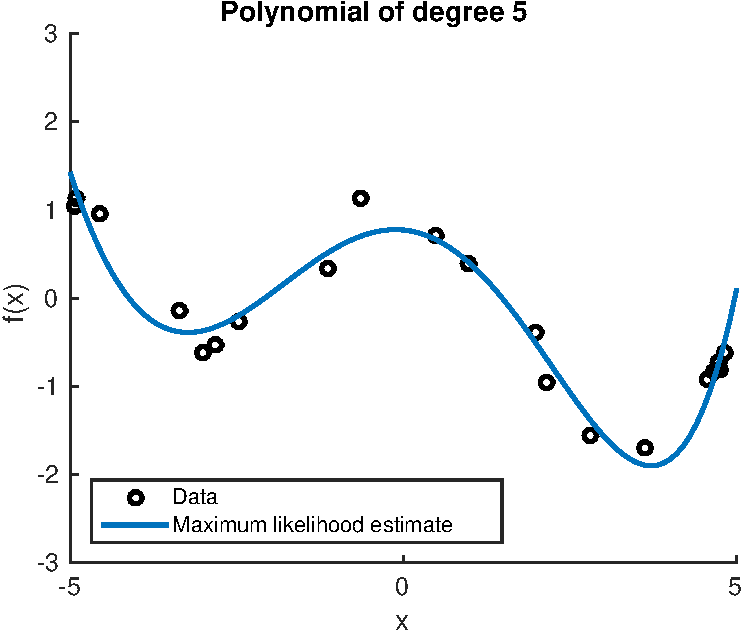
\includegraphics[width = 0.4\hsize]{./figures-intro-curvefitting/polynomial5}
 \end{figure}
 
 \vspace{-1mm}
 \begin{itemize}
 \item \cemph{Training the model} means finding parameters $\vec\theta^*$, such
   that $f(\vec x_i,\vec\theta^*)\approx y_i$
 \item Define a \cemph{loss function}, e.g., $\sum_{i=1}^N(y_i - f(\vec x_i,
   \vec\theta))^2$, which we want to optimize% \\
   % \arrow \cemph{Maximum likelihood estimation} does this implicitly
 \item Adjust $\vec\theta$ until loss is as small as we can get it: \emph{Minimisation} / \emph{optimisation}.
 \end{itemize}
\end{frame}


%%%%%%%%%%%%%%%%%%%%%%%%%%%%%%%%%%%%%%%%%
\begin{frame}{Example: Minimising the loss}
 \begin{figure}
   \centering
   \only<1>{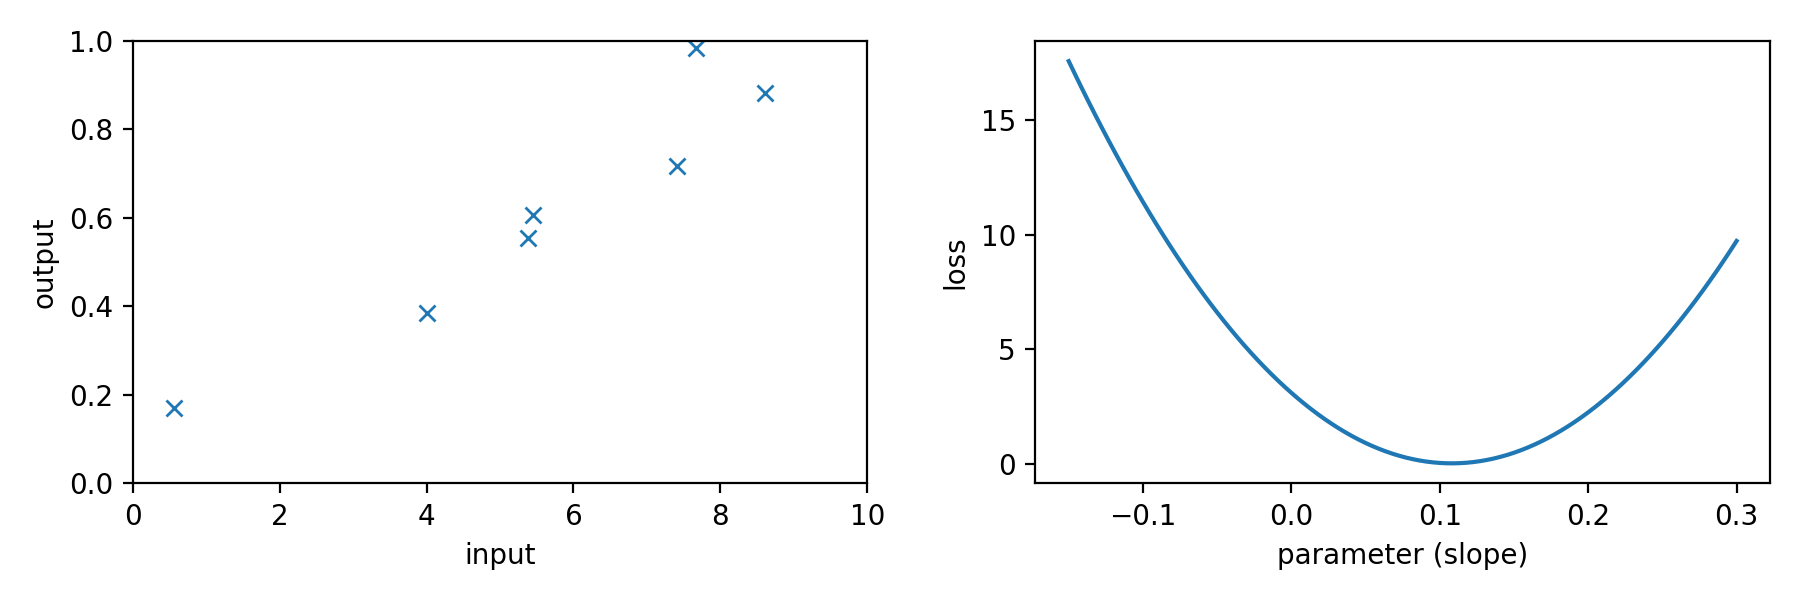
\includegraphics[width=\hsize]{./figures-vectorcalc/linreg-problem.png}}
   \only<2>{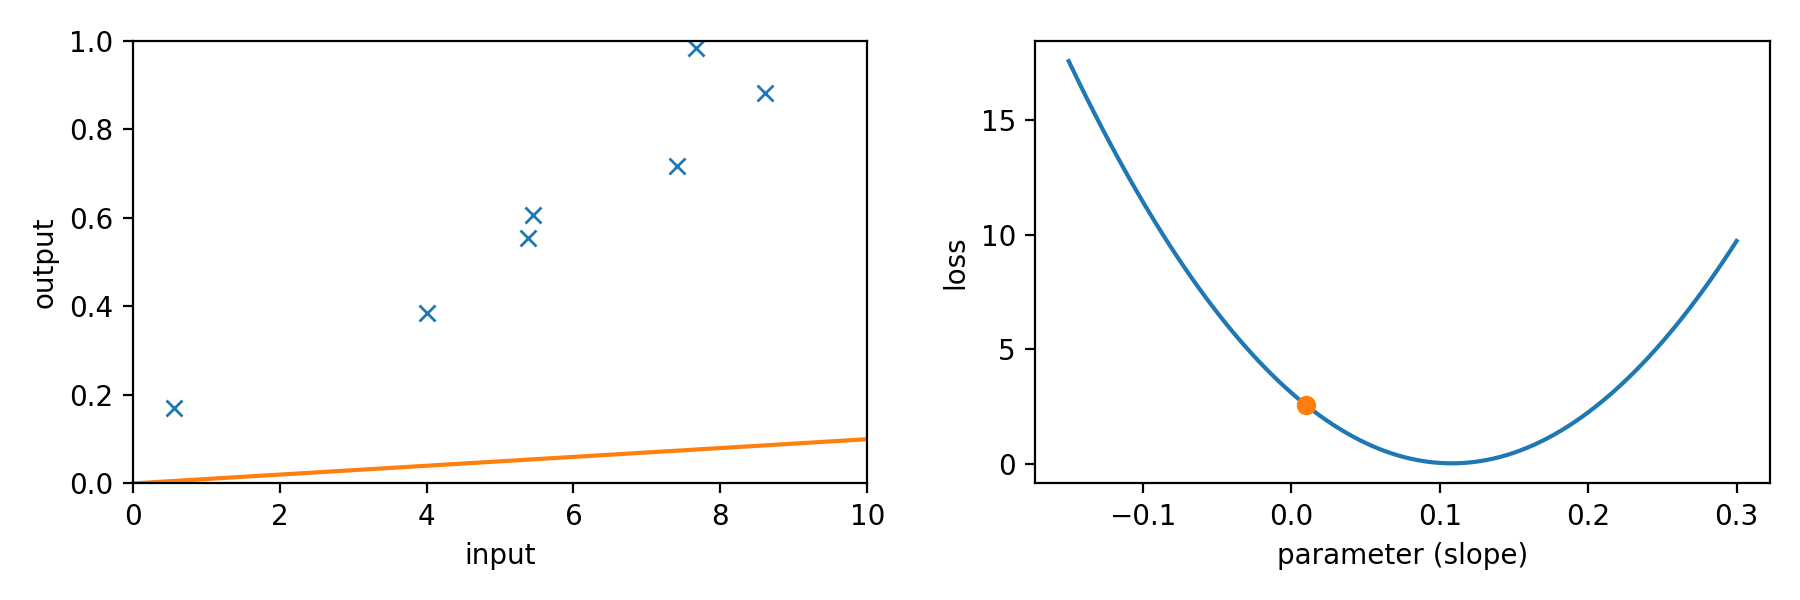
\includegraphics[width=\hsize]{./figures-vectorcalc/linreg-loss-0.png}}
   \only<3>{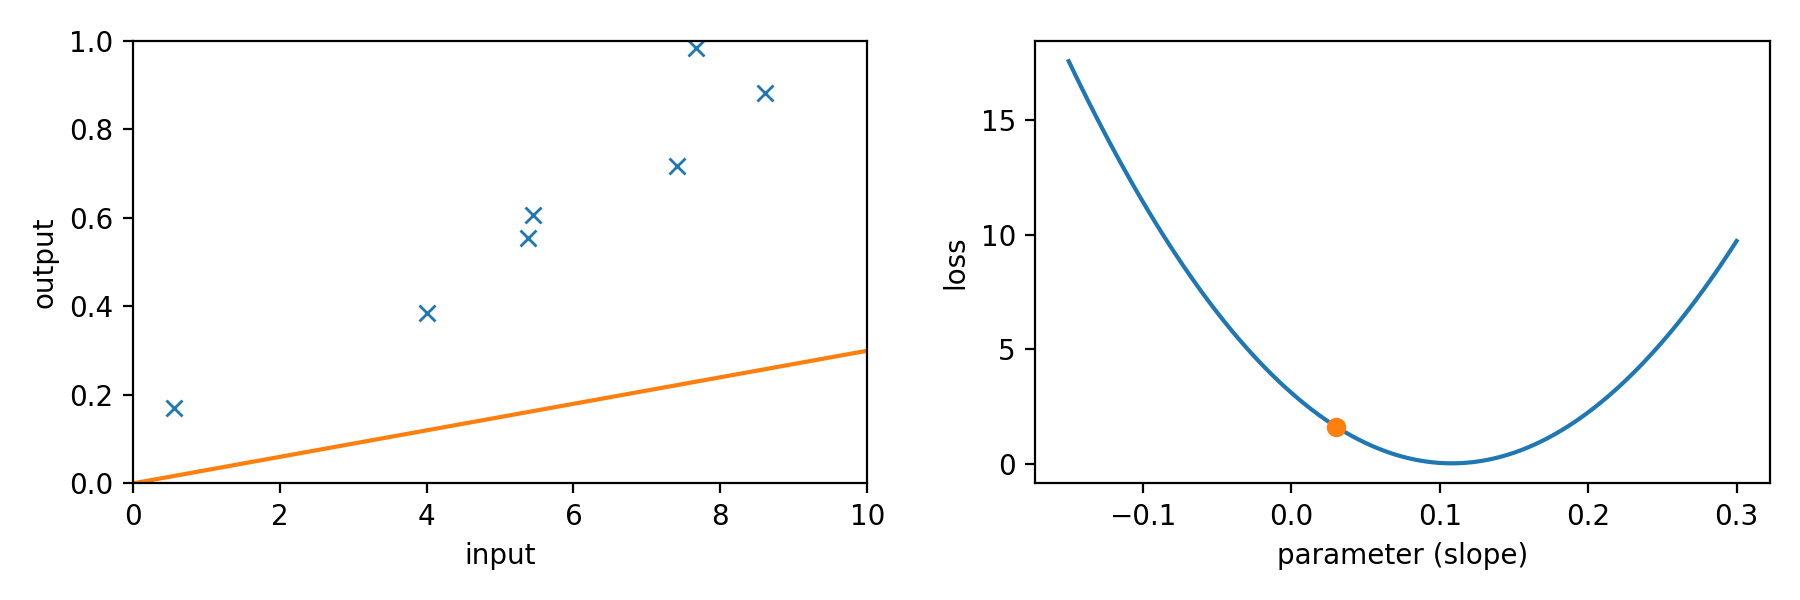
\includegraphics[width=\hsize]{./figures-vectorcalc/linreg-loss-1.png}}
   \only<4>{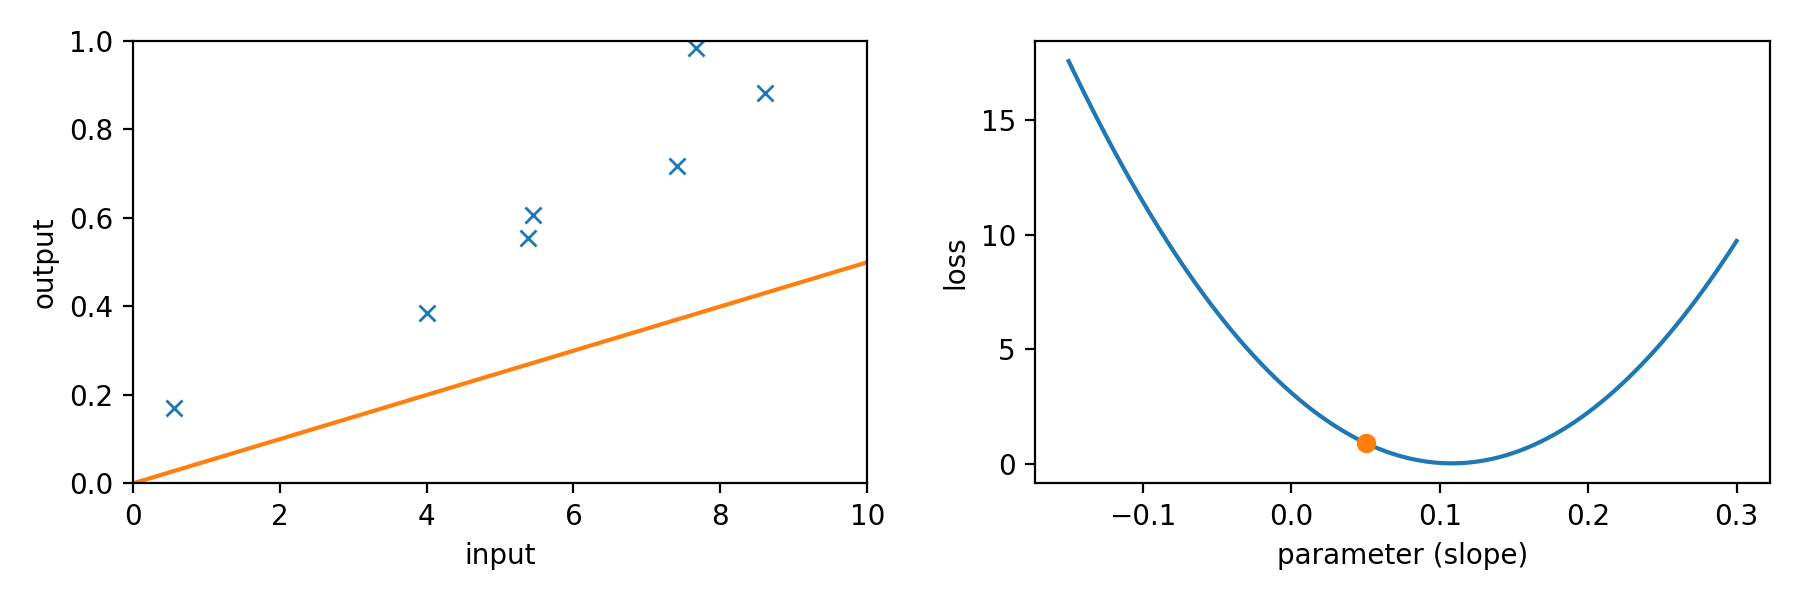
\includegraphics[width=\hsize]{./figures-vectorcalc/linreg-loss-2.png}}
   \only<5>{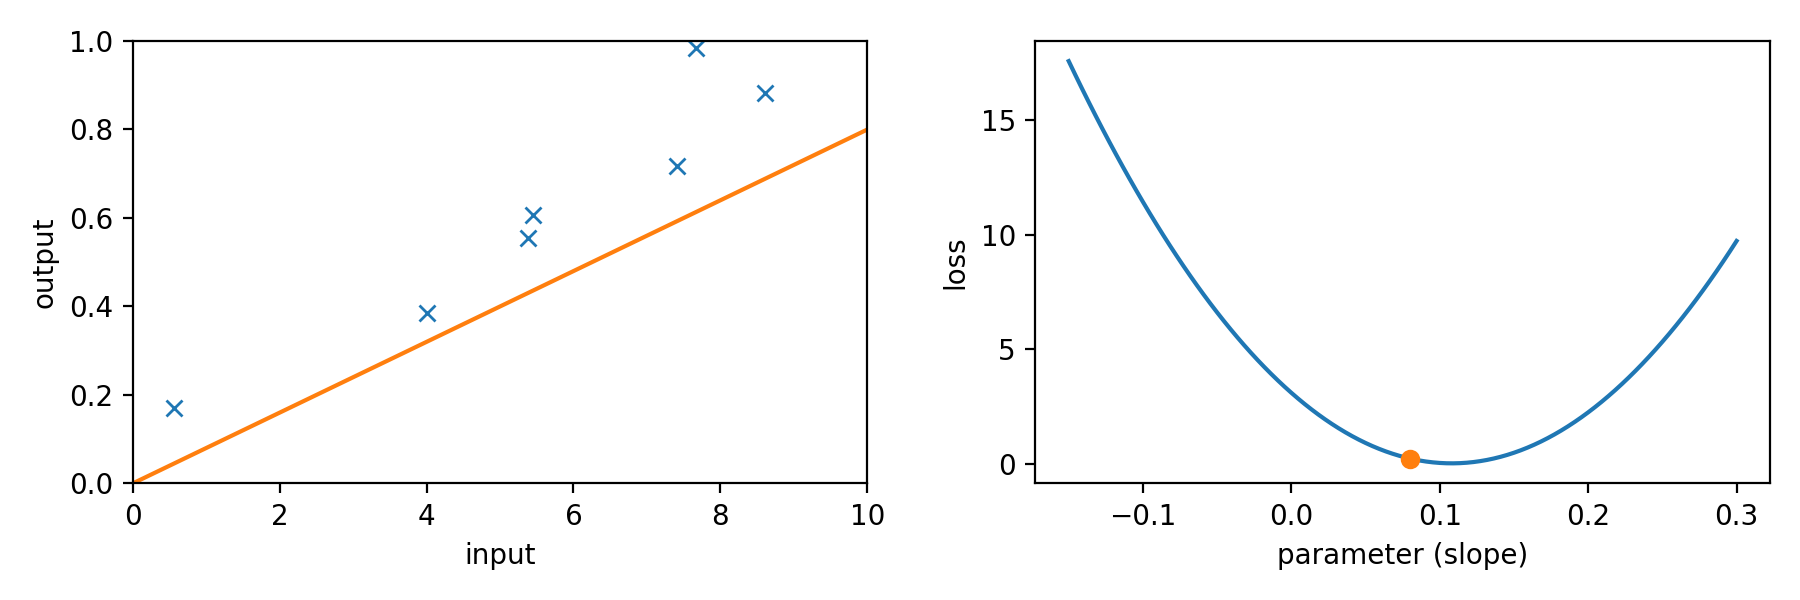
\includegraphics[width=\hsize]{./figures-vectorcalc/linreg-loss-3.png}}
   \only<6>{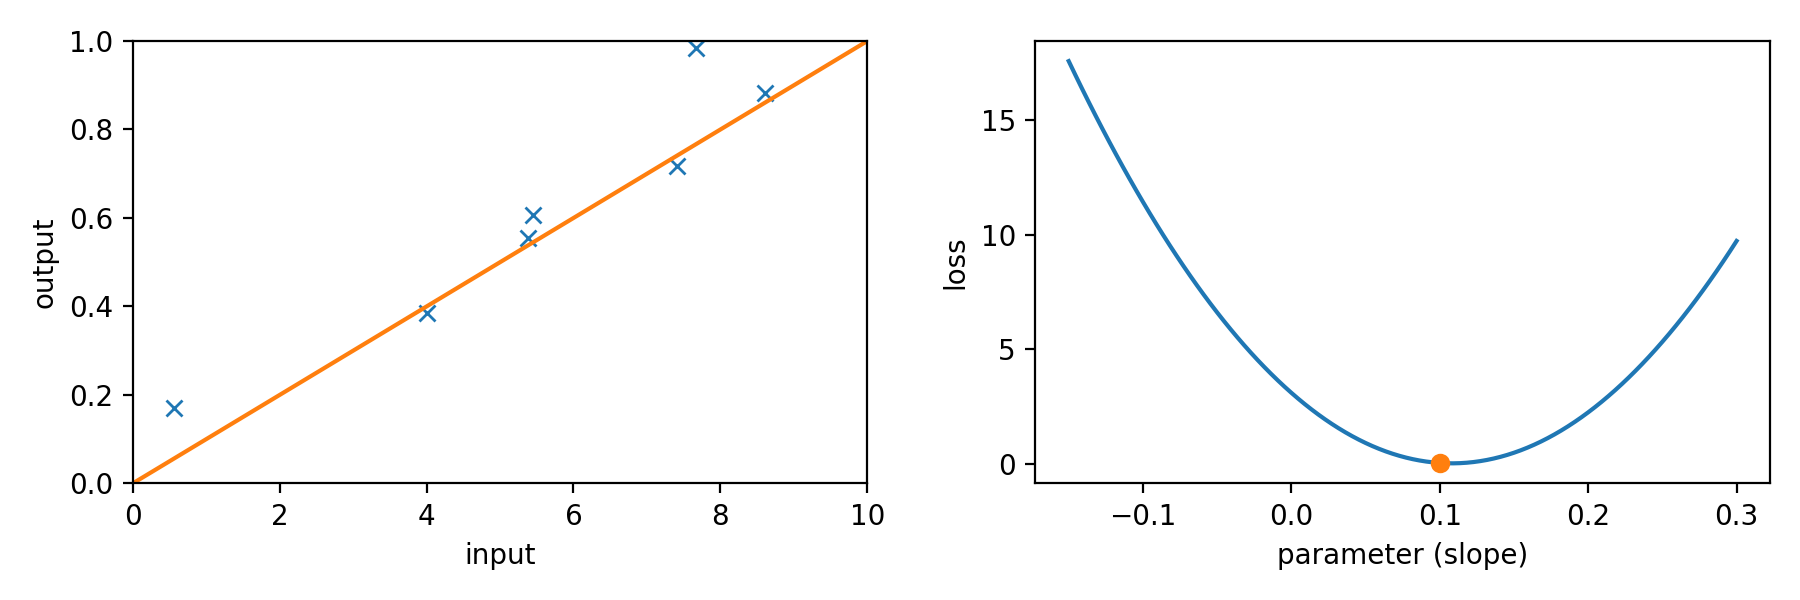
\includegraphics[width=\hsize]{./figures-vectorcalc/linreg-loss-4.png}}
   \only<7>{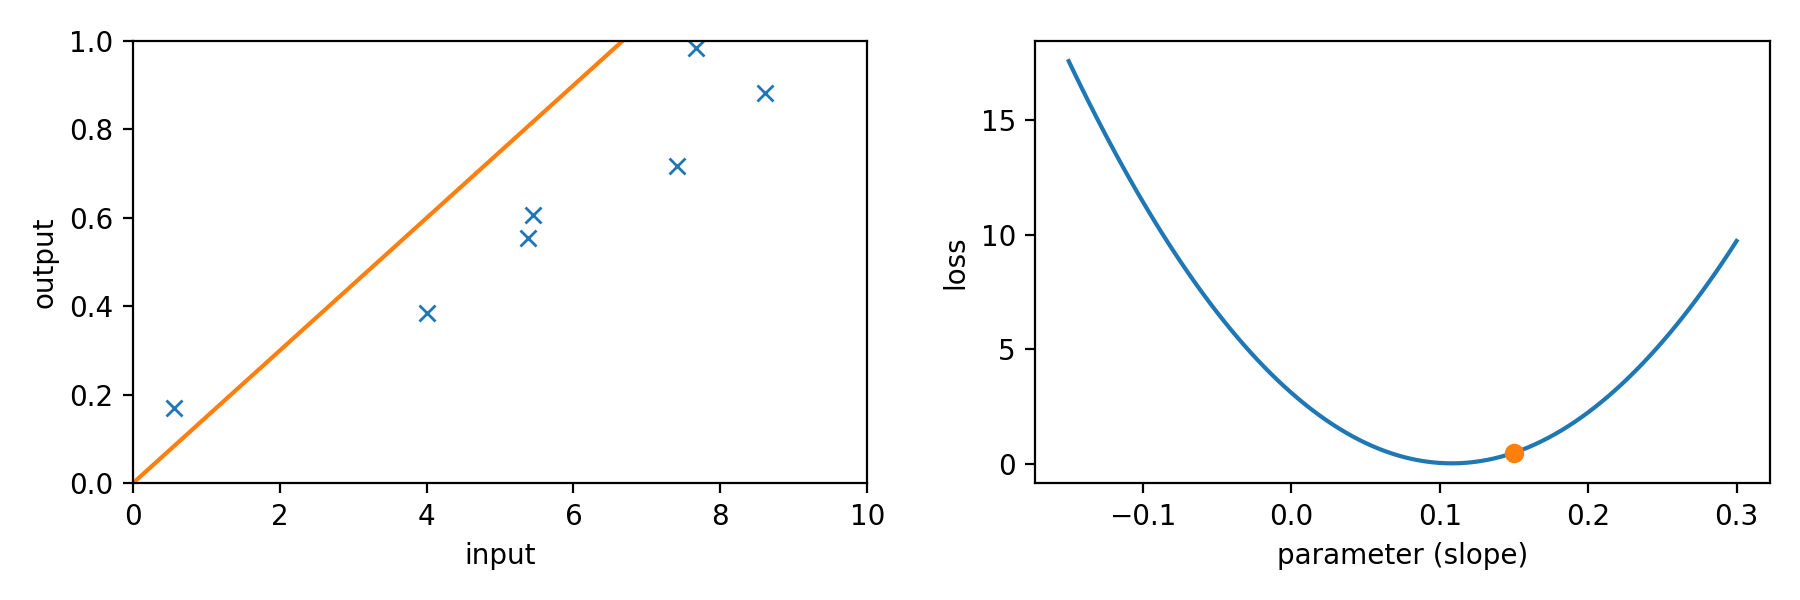
\includegraphics[width=\hsize]{./figures-vectorcalc/linreg-loss-5.png}}
   \only<8>{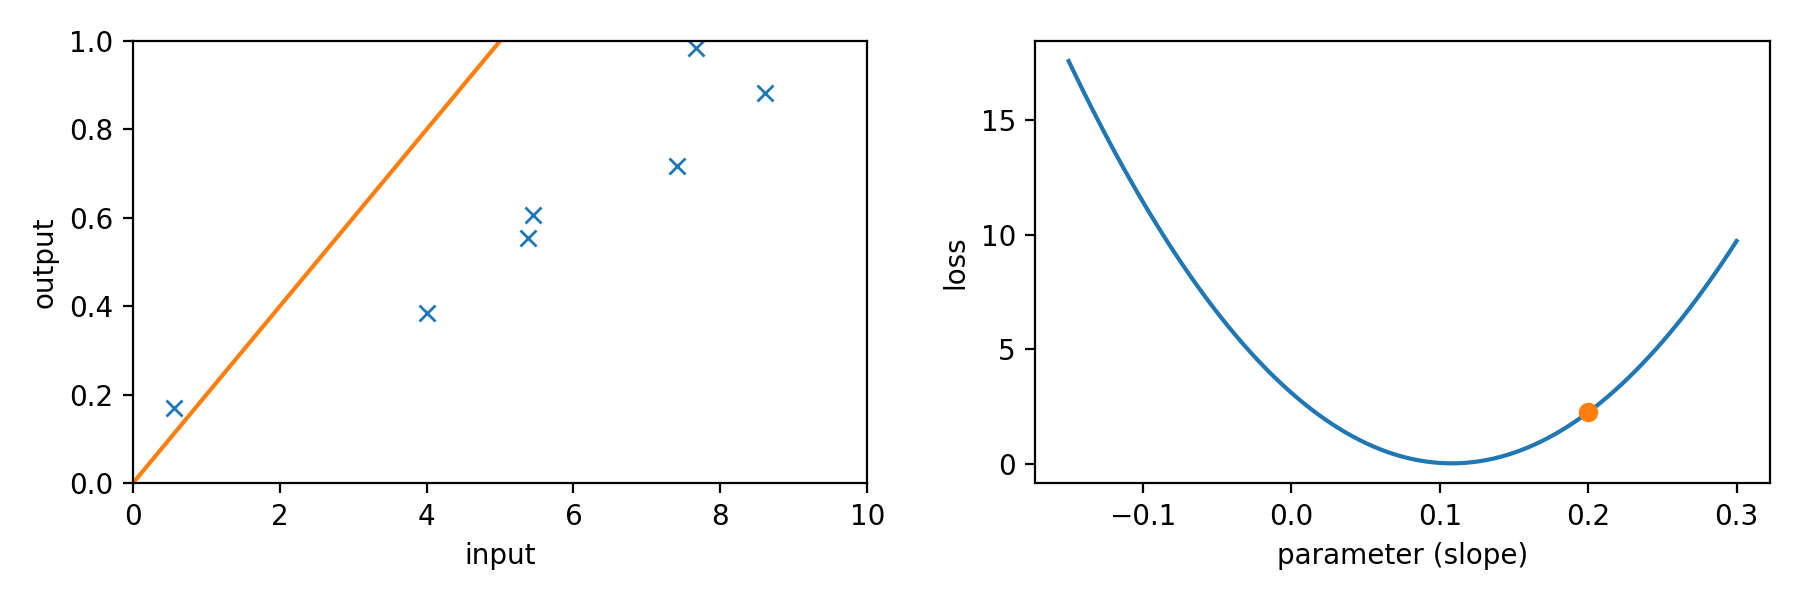
\includegraphics[width=\hsize]{./figures-vectorcalc/linreg-loss-6.png}}
   \only<9>{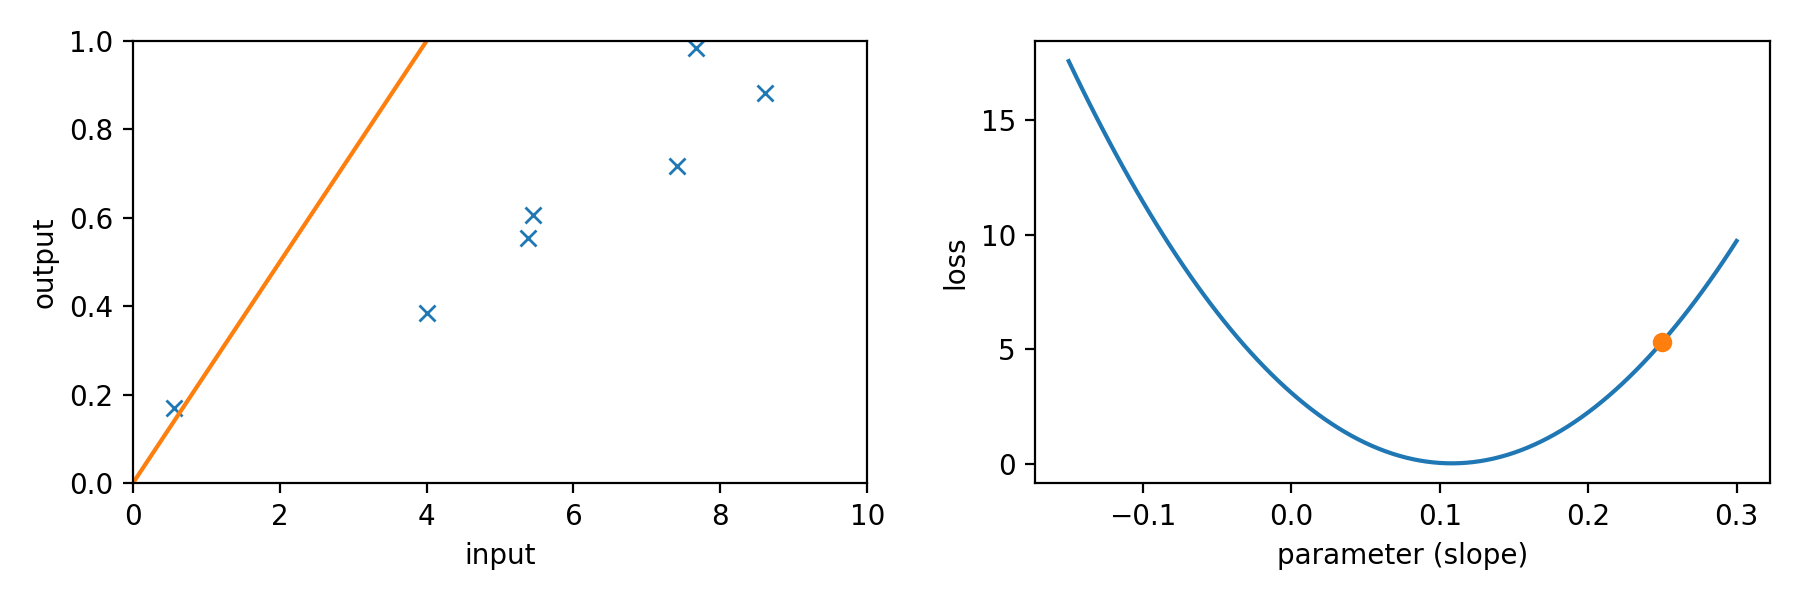
\includegraphics[width=\hsize]{./figures-vectorcalc/linreg-loss-7.png}}
   \only<10>{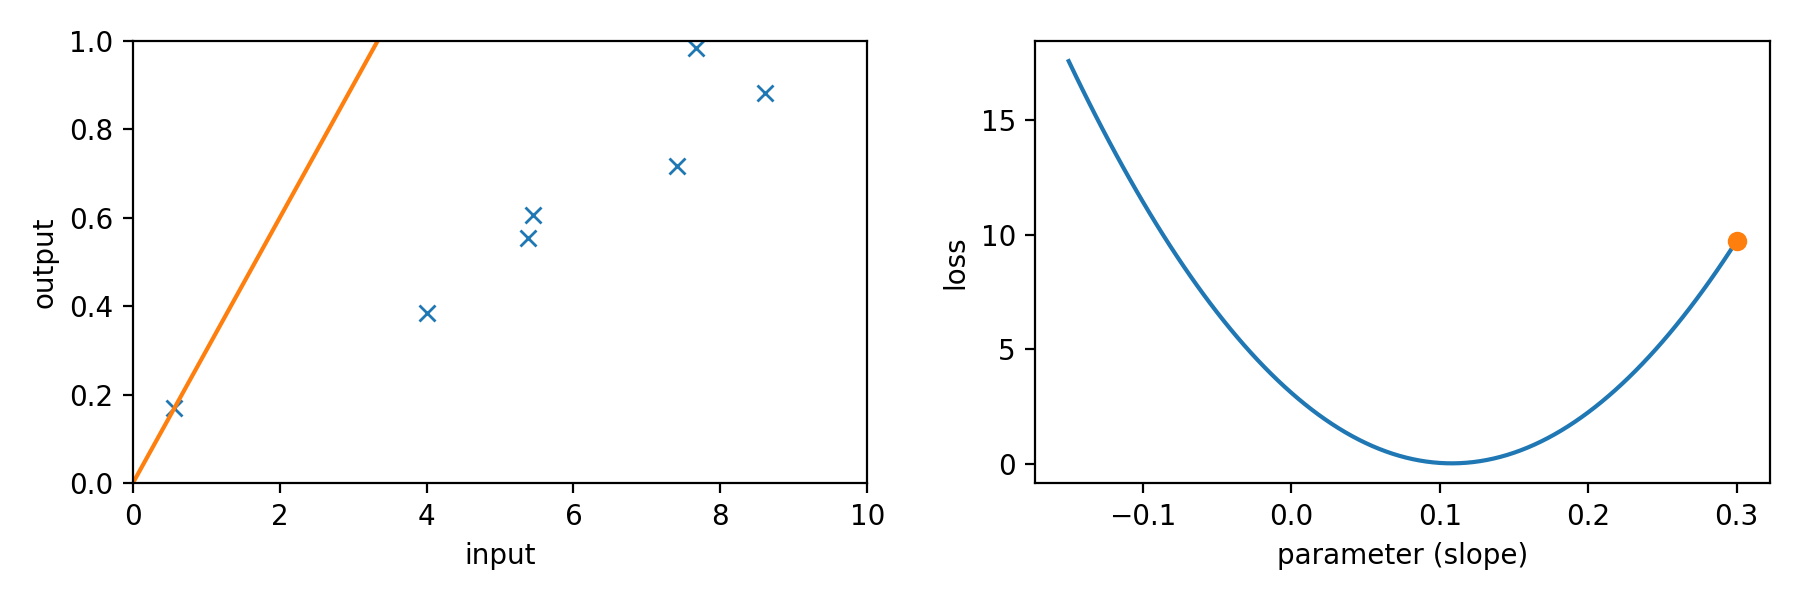
\includegraphics[width=\hsize]{./figures-vectorcalc/linreg-loss-8.png}}
 \end{figure}
\begin{align}
f(x) = a\cdot x && L(a) = \sum_{n=1}^N (f(x_n, a) - y_n)^2
\end{align}
\begin{center}
Let's adjust $a$.
\end{center}
\end{frame}



%%%%%%%%%%%%%%%%%%%%%%%%%%%%%%%%%%%%%%%%%
\begin{frame}{Example: Minimising the loss}
 \begin{figure}
   \centering
   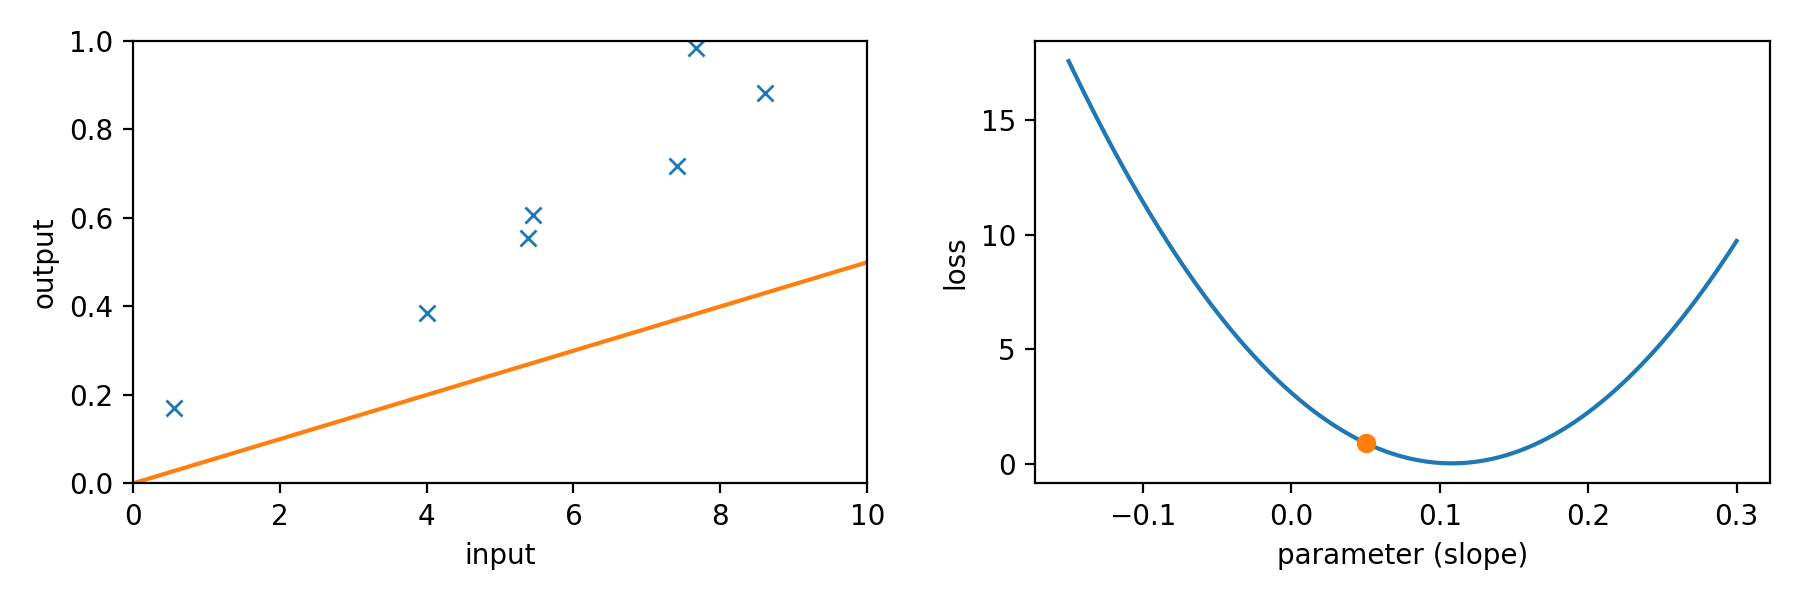
\includegraphics[width=\hsize]{./figures-vectorcalc/linreg-loss-2.png}
 \end{figure}
Two questions for now:
\begin{itemize}
\item How should we change $a$ to make the loss smaller?
\item How do we know when we can't get better?
\end{itemize}
\end{frame}





% \begin{frame}
% \frametitle{Types of Differentiation}

% \begin{enumerate}
% \item Scalar differentiation: $f:\R\to\R$ \\ \qquad \qquad \colchar{$y \in \R \text{ w.r.t. } x \in \R$}{green}
% \item Multivariate case: $f:\R^N\to\R$ \\ \qquad \qquad \colchar{$y \in \R \text{ w.r.t. vector } \vec x \in \R^N$}{green}
% \item Vector fields: $f:\R^N\to\R^M$ \\ \qquad \qquad \colchar{$\text{vector } \vec y \in \R^M \text{ w.r.t. vector } \vec x \in \R^N$}{green}
% \item General derivatives: $f:\R^{M\times N}\to \R^{P\times Q}$ \\
%   \qquad \qquad \colchar{$\text{matrix } \vec y \in \R^{P \times Q}
%     \text{ w.r.t. matrix }\mat X \in \R^{M \times N}$}{green}
% \end{enumerate}


% \end{frame}


\section{Differentiation w.r.t.~scalars}




%%%%%%%%%%%%%%%%%%%%%%%%%%%%%%%%%%%%%%%%%
\begin{frame}
  \frametitle{Scalar Differentiation $f: \R\to\R$}

% \begin{figure}
%   \centering
%   \includegraphics[width = 0.6\hsize]{./figures/finite_differences}
% \end{figure}

\begin{itemize}
\item Derivative defined as the limit of the difference quotient
%
$$
f^\prime(x) = \frac{df}{dx} = \lim_{h\to 0} \frac{f(\colchar{$x + h$}{red}) - f(x)}{h}
$$
\arrow Slope of the secant line through $f(x)$ and
$f(x+h)$
\end{itemize}
\begin{center}
  \animategraphics[loop,
  width=0.6\hsize]{10}{./figures-vectorcalc/finite-diff-animation/finite_diff_step_}{99}{0}
\end{center}

\end{frame}

%%%%%%%%%%%%%%%%%%%%%%%%%%%%%%%%%%%%%%%%%
\begin{frame}
\frametitle{Some Examples}
$$
\begin{array}{ll}
  f(x) = x^n\qquad & f^\prime(x) = nx^{n-1}\\
  f(x) = \sin(x)\qquad & f^\prime(x) = \cos(x)\\
  f(x) = \tanh(x) \qquad& f^\prime(x) = 1-\tanh^2(x)\\
  f(x) = \exp(x) \qquad &f^\prime(x) = \exp(x)\\
  f(x) = \log(x) \qquad &f^\prime(x) = \frac{1}{x}
\end{array}
$$
\end{frame}


%%%%%%%%%%%%%%%%%%%%%%%%%%%%%%%%%%%%%%%%%
\begin{frame}
  \frametitle{Differentiation Rules}

  \begin{itemize}[<+->]
  \item Sum Rule
    $$\big(f(x)+g(x)\big)^\prime = \green{f^\prime(x)} + \blue{g^\prime(x)} =
    \green{\frac{df(x)}{dx}} + \blue{\frac{dg(x)}{dx}}$$
  \item Product Rule
    $$
    \big(f(x) g(x)\big)^\prime = \green{f^\prime(x)g(x)} + \blue{f(x)g^\prime(x)} =
    \green{\frac{df(x)}{dx}g(x)} + \blue{f(x) \frac{d g(x)}{dx}}
    $$
  \item Chain Rule
    $$
     (g\circ f)^\prime(x) =  \big(g(f(x))\big)^\prime
     =\green{g^\prime(f(x))}\blue{f^\prime(x)} = \green{\frac{dg(f(x))}{df}}\blue{\frac{df(x)}{dx}}
    $$
   \item Quotient Rule
   	$$
   	\Big(\frac{f(x)}{g(x)}\Big)^\prime = \frac{\green{f(x)^\prime g(x)} - \blue{f(x)g(x)^\prime}}{\green{(g(x))^2}} = \frac{\blue{\frac{df}{dx}g(x)} - \green{f(x)\frac{dg}{dx}}}{\green{(g(x))^2}}
   	$$
  \end{itemize}
\end{frame}


%%%%%%%%%%%%%%%%%%%%%%%%%%%%%%%%%%%%%%%%%
\begin{frame}
\frametitle{Example: Scalar Chain Rule}
$$
     (g\circ f)^\prime(x) =  \big(g(f(x))\big)^\prime
     =\green{g^\prime(f(x))}\blue{f^\prime(x)} = \green{\frac{dg}{df}}\blue{\frac{df}{dx}}
    $$
    
\begin{columns}[t]

\column{0.50\hsize}
\begin{center}
\textbf{Beginner}
\end{center}
\vspace{-6mm}

\begin{align*}
  g(z) &= 6z + 3\\
  z &= f(x) = -2x + 5 \\
  (g\circ f)^\prime(x) &= \onslide+<2->{\green{\underbrace{(6)}_{dg/df}}\blue{\underbrace{(-2)}_{df/dx}} \\ &= -12}
\end{align*}


\column{0.60\hsize}
\begin{center}
\textbf{Advanced}
\end{center}
\vspace{-6mm}

\begin{align*}
%  f(x) = \frac{\exp(x) + \exp(-x)}{\exp(x)}\\
  g(z) &= \tanh(z)\\
  z &= f(x) = x^n \\
  (g\circ f)^\prime(x) &= \onslide+<2->{\green{\underbrace{\big(1-\tanh^2(x^{n}))}_{dg/df}}\blue{\underbrace{nx^{n-1}}_{df/dx}}}
\end{align*}

\end{columns}
\onslide+<1>{
\vspace{-4mm}
\begin{center}
\textbf{Work it out with your neighbors}
\end{center}}
\end{frame}



\begin{frame}{Finding minima}
\vspace{-0.4cm}
 \begin{figure}
   \centering
   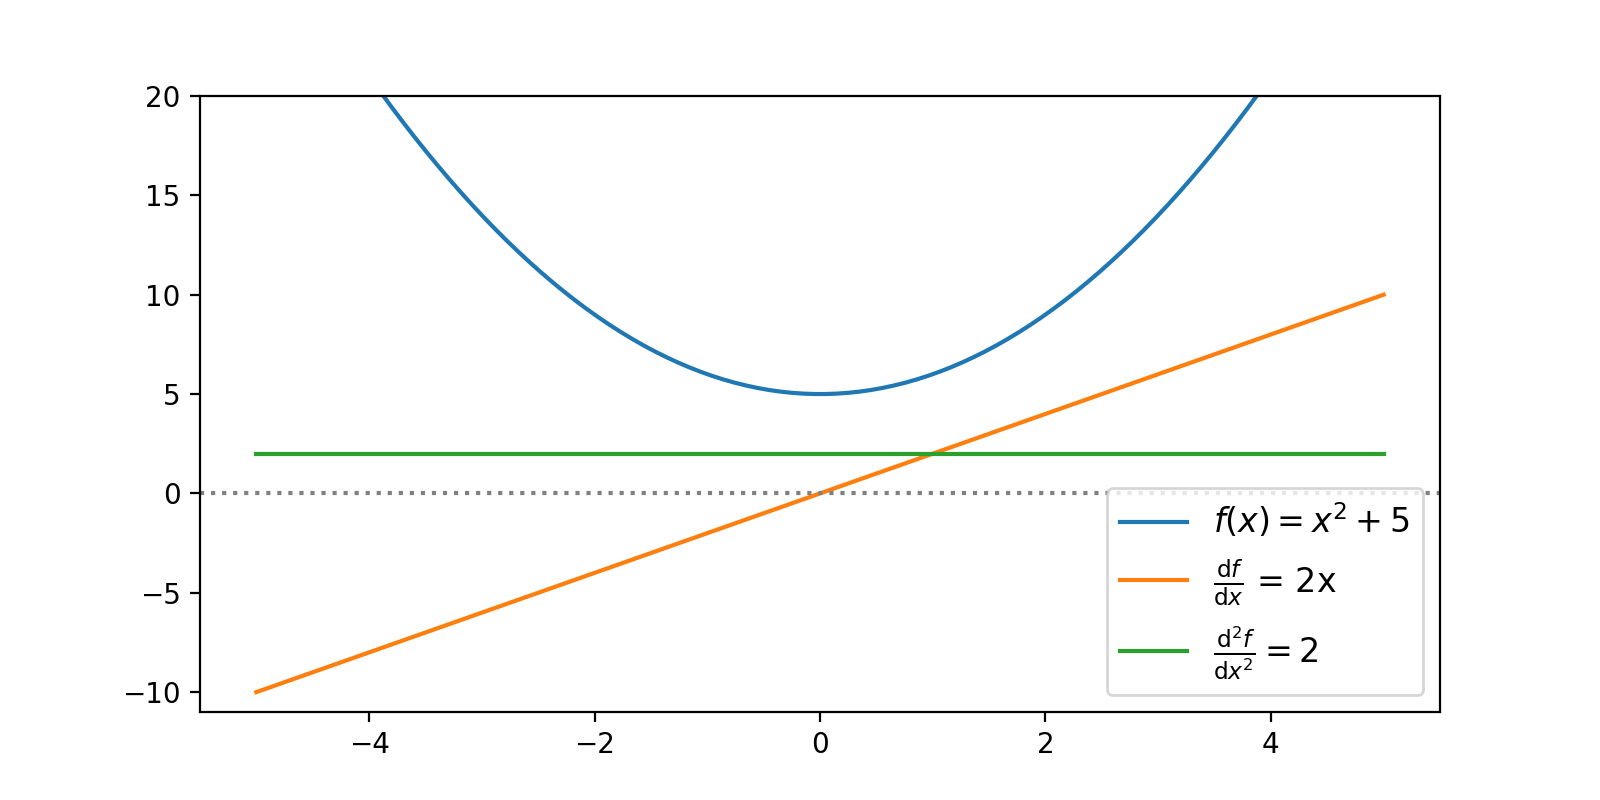
\includegraphics[width=0.85\hsize]{./figures-vectorcalc/gradient-example.png}
 \end{figure}
\vspace{-0.4cm}
Q1: How should we change the input to reduce the output? \pause \\
% The derivative tells us how the function changes if we increase the input. So: \pause
\begin{itemize}
\item Find the derivative function and compute it at a point to find the point's gradient. \pause
\item Increase for negative gradients. Decrease for positive gradients. \pause
\end{itemize}
This is the idea behind \emph{gradient descent}.
\end{frame}



\begin{frame}{Finding minima}
\vspace{-0.4cm}
 \begin{figure}
   \centering
   \only<1,3>{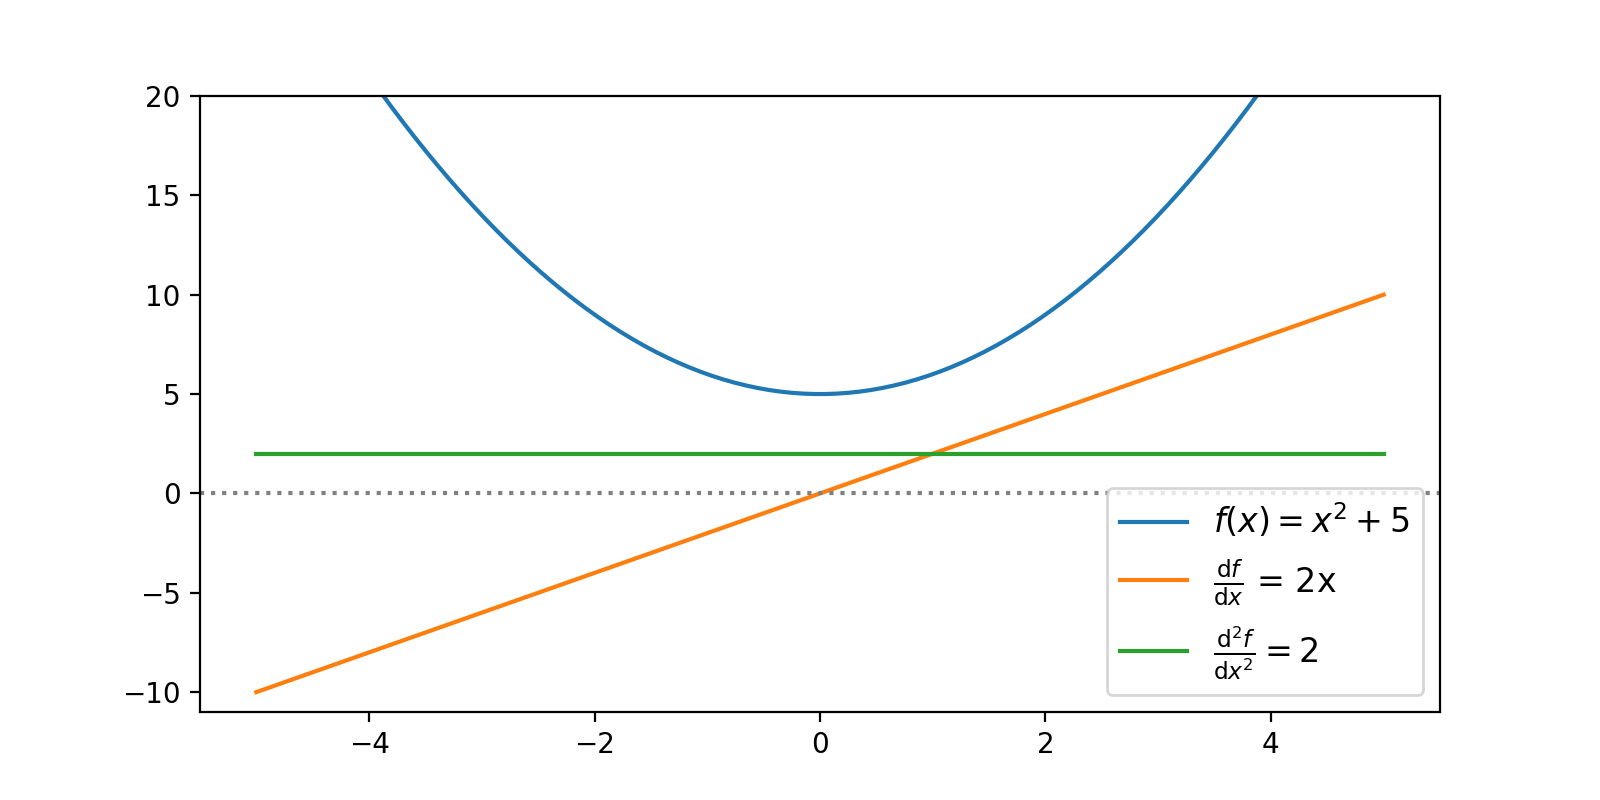
\includegraphics[width=0.85\hsize]{./figures-vectorcalc/gradient-example.png}}
   \only<2>{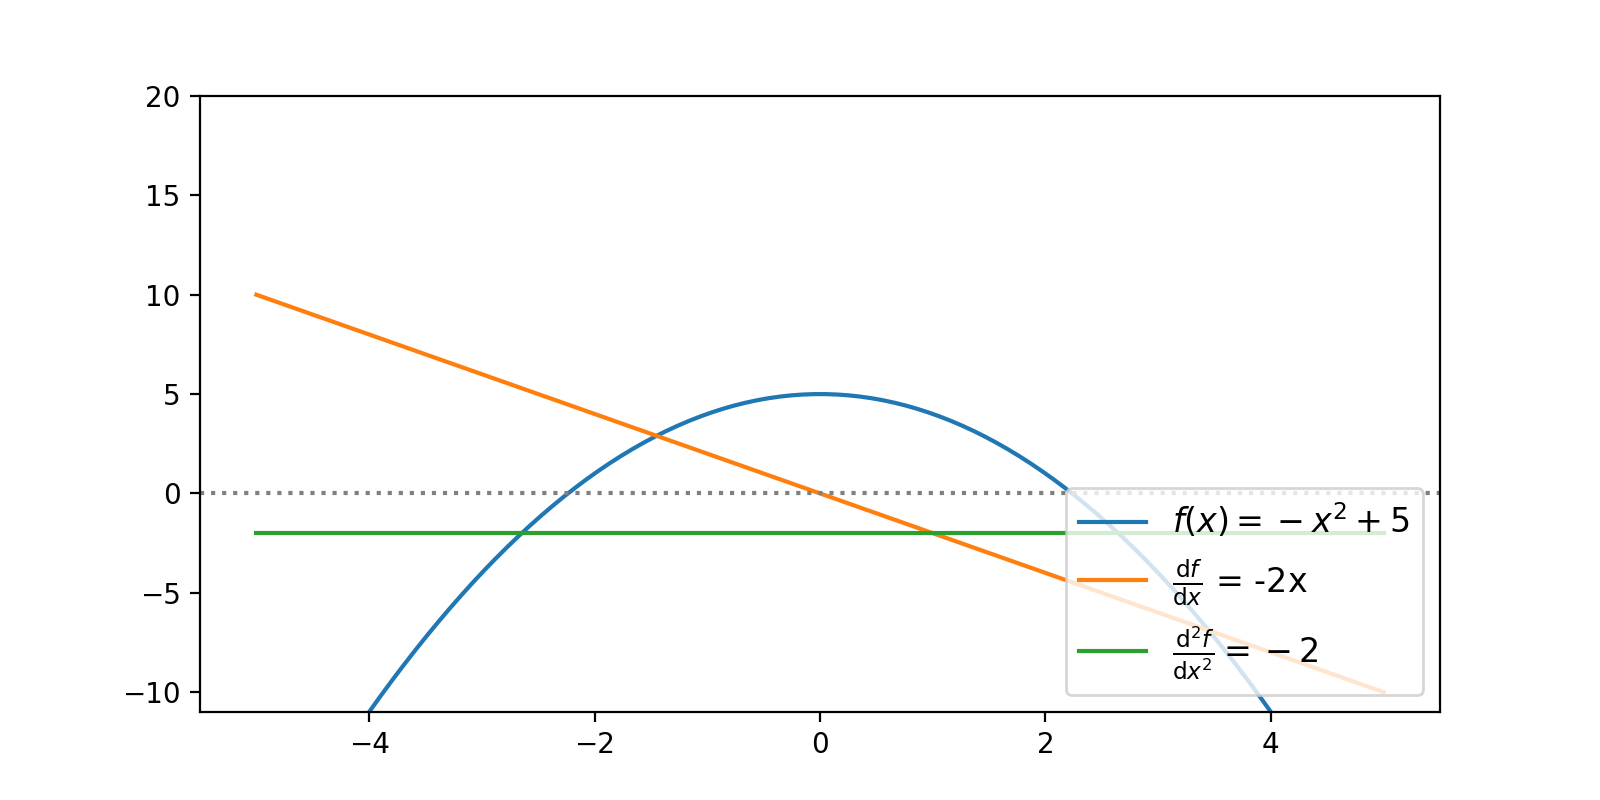
\includegraphics[width=0.85\hsize]{./figures-vectorcalc/gradient-example-max.png}}
 \end{figure}
\vspace{-0.4cm}
\begin{itemize}
\item At a minimum, there is no change we can make that lowers our function value $\implies$ gradient must be zero. \pause
\item Zero gradient is not enough! \pause
\item For minimum, $f(x)$ must go from decreasing to increasing \\
$\implies$ gradient of gradient positive
\end{itemize}
\end{frame}


\begin{frame}{Local and global minima}
Board.
\end{frame}



\begin{frame}{Example: Linear regression}
For the example from earlier, find optimal $a$:
\begin{align}
f(x) = a\cdot x && L(a) = \sum_{n=1}^N (f(x_n) - y_n)^2
\end{align} \pause
\begin{align}
\deriv[L]{a} = \sum_{n=1}^N 2 (a x_n - y_n) x_n = \sum_{n=1}^N 2ax_n^2 - 2x_ny_n = 0
\end{align} \pause
\begin{align}
2a \sum_n x_n^2 = \sum_n2x_ny_n
\end{align} \pause
\begin{align}
a = \frac{\sum_nx_ny_n}{\sum_n x_n^2}
\end{align} \pause
\begin{align}
\frac{\mathrm{d}^2L}{\mathrm{d}a^2} = \sum_{n=1}^N 2x_n^2 \geq 0
\end{align}
\end{frame}


\begin{frame}{Summary}
You have seen:
\begin{itemize}
\item That derivatives are useful for finding minima of functions \pause
\item How to differentiate simple functions \pause
\item An example of solving for the minimum point \pause
\item How to identify minima \pause
\end{itemize}

% Consider exercises 5.1-5.3 in the MML book. EXERCISES
\end{frame}

\section{Differentiation w.r.t.~vectors}

\begin{frame}{Linear regression: multiple parameters}
What happens when our function has multiple parameters?
\begin{equation}
f(x) = \theta_3 x^3 + \theta_2 x^2 + \theta_1 x + \theta_0
\end{equation} \pause

Think of a \emph{vector} as parameterising our function:
\begin{align}
f(x) = \vec\theta\transpose \vphi(x) && \vphi(x) = \begin{bmatrix}x^3 && x^2 && x && 1\end{bmatrix}\transpose
\end{align} \pause

We want to:
\begin{itemize}
\item Understand how a function (e.g.~loss) changes when we change $\vec\theta$. \pause
\item Characterise what an optimum is for a function of a vector.
\end{itemize} \pause

\begin{center}
Both can be analysed by \\ turning the multi-D problem into many 1D problems.
\end{center}
\end{frame}

\begin{frame}{Directional derivative}

 \begin{figure}
   \centering
   \includegraphics[width=0.7\hsize]{./figures-vectorcalc/directional-deriv.png}
 \end{figure}

 How does the function change if we move in a particular \textit{direction}?
\end{frame}

\begin{frame}{Directional derivative}
Define \emph{directional derivative} $\nabla_\vv L(\vtheta)$ as how much the function changes if we move in direction $\vv$:
\only<1>{
\begin{align*}
\nabla_\vv L(\vtheta) = \lim_{h\to 0} \frac{L(\vtheta + h\vv) - L(\vtheta)}{h}
\end{align*}}
\only<2->{\begin{equation*}
\nabla_\vv L(\vtheta) = \lim_{h\to 0} \frac{L(\theta_1 + hv_1, \theta_2 + hv_2) - L(\theta_1, \theta_2)}{h}
\end{equation*}} \pause\pause
\begin{equation*}
= \lim_{h\to 0} \frac{L(\theta_1 + hv_1, \theta_2 + hv_2) - {\color{blue}L(\theta_1, \theta_2  + hv_2)}}{h} + \frac{{\color{blue}L(\theta_1, \theta_2 + hv_2)} - L(\theta_1, \theta_2)}{h}
\end{equation*}\pause
\begin{equation*}
= \lim_{h\to 0} \frac{L(\theta_1 + h', \theta_2 + h'\frac{v_2}{v_1})\!-\!{\color{blue}L(\theta_1, \theta_2  + h'\frac{v_2}{v_1})}}{h'/v_1}\!+\! \frac{{\color{blue}L(\theta_1, \theta_2 + h'')}\!-\!L(\theta_1, \theta_2)}{h''/v_2}
\end{equation*}\pause
\begin{equation*}
= \pderiv[L]{\theta_1} v_1 + \pderiv[L]{\theta_2} v_2% && \qquad \text{to prove, substitute e.g.~}h' = hv_1
\end{equation*} \pause
\begin{itemize}
\item Can find gradient in \emph{any} direction with the \emph{partial derivatives} \pause
% \item An optimum is where the gradient is zero in \emph{all directions}!
\end{itemize}
\end{frame}


%%%%%%%%%%%%%%%%%%%%%%%%%%%%%%%%%%%%%%%%%
\begin{frame}
  \frametitle{Multivariate Differentiation $f: \R^N\to\R$}

  \begin{align*}
    y = f(\vec x)\,,\quad \vec x =\begin{bmatrix}
                                    x_1\\
                                    \vdots\\
                                    x_N
                                  \end{bmatrix}\in\R^N
  \end{align*}

  \begin{itemize}[<+->]
  \item \cemph{Partial derivative} (change one coordinate at a time):
    \begin{align*}
      \frac{\partial f}{\partial x_i} = \lim_{h\to 0}
      \frac{f(x_1,\dotsc, x_{i-1}, \colchar{$x_i + h$}{red}, x_{i+1},
      \dotsc, x_N) - f(\vec x)}{h}
    \end{align*}
  \item \cemph{Jacobian} vector (\cemph{gradient}) collects all partial derivatives:
    \begin{align*}
      \diffF{f}{\vec x} =
      \begin{bmatrix}
         \frac{\partial f}{\partial x_1} & \cdots & \pdiffF{f}{x_N}
      \end{bmatrix}\in\R^{1\times N}
    \end{align*}
    Note: This is a \emph{row vector}.
  \end{itemize}
  
\end{frame}


\begin{frame}{Steepest descent direction}
Directional derivative:
\begin{equation}
\nabla_{\vec v} f(\vtheta) = \diffF{f}{\vtheta}\vec v
\end{equation}
\vspace{-0.5cm}
\begin{center}\small(inner product, row vector times column vector)\end{center} \pause

\vspace{0.2cm}

\begin{center}
\large What is the direction where the function changes the most?
\end{center} \pause
\begin{equation}
\diffF{f}{\vtheta}\vec v = \norm{\diffF{f}{\vtheta}}\norm{\vec v} \cos \beta 
\end{equation}\pause
\begin{itemize}
\item Choose unit vector $\vec v$ \pause
\item Angle between vectors $\beta$ should be zero $\implies \cos \beta = 1$. \pause
\end{itemize}
\begin{center}
\Large Steepest descent points in direction of Jacobian/gradient vector.
\end{center}
\end{frame}


%%%%%%%%%%%%%%%%%%%%%%%%%%%%%%%%%%%%%%%%%
\begin{frame}[t]
\frametitle{Example: Multivariate Differentiation}

\vspace{-1cm}
\begin{columns}[t]

\column{0.50\hsize}
\begin{center}
\textbf{Beginner}
\end{center}
\vspace{-6mm}

\begin{align*}
  &f: \R^2 \to \R\\
  &f(x_1,x_2) = x_1^2x_2+x_1x_2^3\in\R
\end{align*}

\column{0.50\hsize}
\begin{center}
\textbf{Advanced}
\end{center}
\vspace{-6mm}

\begin{align*}
 &f: \R^2 \to \R\\
  &f(x_1,x_2) = (x_1 + 2x_2^3)^2\in\R
\end{align*}

\end{columns}

\begin{center}
Partial derivatives\visible<1>{? Gradient?}  \\
\visible<1>{\textbf{Work it out with your neighbors}}
\end{center}
\vspace{-1.35cm}

\pause
\begin{columns}[t]

\column{0.5\hsize}
\begin{align*}
\frac{\partial f(x_1,x_2)}{\partial x_1} &= 2x_1x_2 + x_2^3\\
\frac{\partial f(x_1,x_2)}{\partial x_2} &= x_1^2+3x_1x_2^2
\end{align*}

\column{0.5\hsize}
\vspace{-4mm}
\begin{align*}
\frac{\partial f(x_1,x_2)}{\partial x_1} &= 2(x_1 + 2x_2^3)\green{\overbrace{(1)}^{\pdiffF{}{x_1}(x_1 + 2x_2^3)}}\\
\frac{\partial f(x_1,x_2)}{\partial x_2} &= 2(x_1 + 2x_2^3)\blue{\underbrace{(6x_2^2)}_{\pdiffF{}{x_2}(x_1 + 2x_2^3)}}\\
\end{align*}

\end{columns}

\pause
\vspace{-1cm}
\begin{align*}
\text{Gradient}\qquad
\diffF{f}{\vec x} =
  \begin{bmatrix}
\frac{\partial f(x_1,x_2)}{\partial x_1} & \frac{\partial
  f(x_1,x_2)}{\partial x_2}
\end{bmatrix} \in\R^{1\times 2}\,
\end{align*}
\vspace{-1.35cm}

\begin{columns}[t]

\column{0.5\hsize}
\begin{align*}
  \diffF{f}{\vec x} =
\begin{bmatrix}
 2x_1x_2 + x_2^3 & x_1^2+3x_1x_2^2
\end{bmatrix}
\end{align*}

\column{0.5\hsize}
\begin{align*}
  \diffF{f}{\vec x} =
\begin{bmatrix}
 2(x_1 + 2x_2^3) & 12(x_1 + 2x_2^3)x_2^2
\end{bmatrix}
\end{align*}

\end{columns}

\end{frame}


\begin{frame}{Optima, minima, maxima}
What is an optimum for a function of a vector?
 \begin{figure}
   \centering
   \includegraphics[width=0.5\hsize]{./figures-vectorcalc/directional-deriv.png}
 \end{figure} \pause
\begin{itemize}
\item Directional derivative should be zero \textit{in all directions} $\implies \diffF{f}{\vec x} = {\vec 0}$. \pause
\item For minimum: second directional derivative should be positive \textit{in all directions}.
\end{itemize}
\end{frame}


\begin{frame}{Summary}
Motivation: Want to optimise functions of several variables \\
\vspace{0.2cm}

% Q1: Understand how function changes when we change vector input. \\
% A1: Directional derivative, found from partial derivatives \\
% \vspace{0.2cm}

% Q2: 
\begin{itemize}
\item Directional derivative
\item Partial derivatives $\implies$ gradient vector
\item Steepest descent direction
\item At an optimum $\diffF{f}{\vec x} = \vec 0$
\end{itemize}
\end{frame}









% \section{Differentiation of vector-valued functions}




% \begin{frame}
%   \frametitle{Chain Rule}
% Back to our linear regression problem:
% \begin{equation}
% L(\vtheta) = \sum_{n=1}^N (y_n - \vphi(x_n)\transpose\vtheta)^2 = ||\vy - \Phi(X)\vtheta||^2
% \end{equation}

% \pause
% \begin{itemize}
% \item We could manually take partial derivatives of $L(\vtheta)$ \pause
% \item Or, we could see our scalar function $L(\vtheta)$ as a function composition:
% \end{itemize}
% \begin{align*}
% f(\vec g(\vtheta)) && f: \Reals^{D}\to\Reals \,, \qquad \vec g: \Reals^{E}\to\Reals^D
% \end{align*}
% \pause
% \vspace{-0.4cm}
% \begin{itemize}
% \item Wouldn't it be nice to have a chain rule? \pause $\diffF{f(\vec g(\vtheta))}{\vtheta} = \diffF{f}{\vec g}\diffF{\vec g}{\vtheta}$ \pause
% \item But how does a derivative of a vector w.r.t.~a vector work?
% \end{itemize}
% \end{frame}


% \begin{frame}{Multivariate Chain Rule w.r.t.~scalar}
% It turns out, there is a multivariate chain rule:
% \only<1>{
% \begin{align*}
% \deriv[f(a(t), b(t))]{t} = \pderiv[f]{a}\deriv[a]{t} + \pderiv[f]{b}\deriv[b]{t}
% \end{align*}}
% \only<2->{
% \begin{align*}
% \deriv[f(\vec g(t))]{t} = \sum_{i=1}^D\pderiv[f]{g_i}\deriv[g_i]{t} && \vec g(t) \in \Reals^D
% \end{align*}} \pause \pause
% This is an inner product. Can write in vector form:
% \begin{align*}
% \deriv[f(\vec g(t))]{t} = \underbrace{\deriv[f]{\vec g}}_{\text{row}}\cdot\underbrace{\deriv[\vec g]{t}}_{\text{column}}
% \end{align*} \pause
% \begin{itemize}
% \item $\deriv[\vec g]{t}$ is the derivative of a column vector. We keep this to be a column vector.
% \item Can also be derived from a limit argument, like the scalar derivative.
% \end{itemize}
% \end{frame}


% \begin{frame}
%   \frametitle{Example: Chain Rule}
%   \begin{itemize}
%     \item 
%   Consider $f:\R^2\to \R, \quad \vec x:\R \to \R^2$
%   \begin{align*}
%     f(\vec x)&= f(x_1, x_2) = x_1^2+2x_2\,,\\
%     \vec x(t) &=
%                 \begin{bmatrix}
%                   x_1(t)\\ x_2(t)
%                 \end{bmatrix} =
%                 \begin{bmatrix}
%       \sin(t)\\ \cos (t)
%     \end{bmatrix}
%   \end{align*}
%   \vspace{-2mm}
%   \pause
% \item What are the dimensions of \blue{$\diffF{f}{\vec x}$} and \red{$\diffF{ \vec x}{t}$}?\\
%   \only<2>{\qquad \qquad \qquad \emph{Work it out with your neighbors}}
%   \pause \qquad \qquad \qquad \qquad \qquad \blue{$1\times 2$} and \red{$2\times 1$}
% \item Compute the gradient $\diffF{f}{t}$ using the chain rule:
%   \pause
%   \begin{align*}
%     \diffF{ f}{t} = \blue{\diffF{f}{\vec x}} \red{\diffF{\vec x}{t}}
%      &= \blue{\begin{bmatrix}
% 		\frac{\partial f}{\partial x_1} & 
% 		\frac{\partial f}{\partial x_2}
% 		\end{bmatrix}}
% 		\red{\begin{bmatrix}
%     	\frac{\partial x_1}{\partial t}\\[2mm]
%         \frac{\partial x_2}{\partial t}
%      	\end{bmatrix}}
%  	= \blue{\begin{bmatrix}
% 		2\sin t & 2
% 		\end{bmatrix}}
%         \red{\begin{bmatrix}
%         \cos t\\
%         -\sin t
%         \end{bmatrix}}\\
%      &= 2\sin t\cos t - 2\sin t = 2\sin t(\cos t -1)
%   \end{align*}
% \end{itemize}
% \end{frame}


% \begin{frame}{Example: Vector Differentiation}
% See jamboard on video.
% \end{frame}



% \begin{frame}{Multivariate Chain Rule w.r.t.~vector}
% Remember: Differentiation w.r.t.~a vector just requires \emph{collecting all partial derivatives}.
% Same chain rule for a single partial deriv:
% \begin{align*}
% \pderiv[f(\vec g(\vx))]{x_j} = \sum_{i=1}^D\pderiv[f]{g_i}\pderiv[g_i]{x_j} && \vec g(\vx) \in \Reals^D
% \end{align*}
% \pause
% This is a matrix multiplication! Can write in vector form:
% \begin{align*}
% \deriv[f(\vec g(\vx))]{\vx} = \underbrace{\deriv[f]{\vec g}}_{\text{row}}\cdot\underbrace{\deriv[\vec g]{\vx}}_{\text{matrix}}
% \end{align*} \pause
% \begin{itemize}
% \item $\deriv[\vec g]{\vx}$ is the derivative of a column vector w.r.t.~the input vector $\vx$. We put the elements of $\vec g$ (i.e.~i) along the column, and the dimensions of the derivative (i.e.~j) along the row. \pause
% \item Can also be derived from a directional derivative argument, but for a vector.
% \end{itemize}
% \end{frame}


% \begin{frame}
%   \frametitle{Vector Field Differentiation $f: \R^N\to\R^M$}
%   \begin{align*}
%     \vec y &= \vec f(\vec x) \in\R^M\,,\quad \vec x \in \R^N\\
%     \begin{bmatrix}
%      \colchar{$ y_1$}{red}\\
%      \vdots\\
%      \colchar{$y_M$}{blue}
%     \end{bmatrix}
%     &=
%     \begin{bmatrix}
%       \colchar{$f_1(\vec x)$}{red}\\
%       \vdots\\
%       \colchar{$f_M(\vec x)$}{blue}
%     \end{bmatrix}
%     =
%     \begin{bmatrix}
%       \colchar{$f_1(x_1,\dotsc, x_N)$}{red}\\
%       \vdots\\
%       \colchar{$f_M(x_1,\dotsc, x_N)$}{blue}
%     \end{bmatrix}
%   \end{align*}
  
%   \pause
%   \begin{itemize}    
%     \item \cemph{Jacobian} matrix (collection of all partial derivatives)
%       \begin{align*}
%         \begin{bmatrix}
%           \colchar{$\frac{d y_1}{d\vec x}$}{red}\\
%           \vdots\\
%           \colchar{$\frac{d y_M}{d\vec x}$}{blue}
%         \end{bmatrix}
%         =
%         \begin{bmatrix}
%           \colchar{$\frac{\partial f_1}{\partial
%               x_1}$}{red} &
%           \cdots & \colchar{$\frac{\partial
%               f_1}{\partial x_N}$}{red}\\
%           \vdots &  & \vdots\\
%           \colchar{$\frac{\partial f_M}{\partial x_1}$}{blue} & \cdots & \colchar{$\frac{\partial
%             f_M}{\partial x_N}$}{blue}
%         \end{bmatrix}
%                                                        \in\R^{M\times N}
%       \end{align*}
%     \end{itemize}
  
% \end{frame}


% \begin{frame}{Dimensionality of the Gradient}
%   In general: A function $\vec
%   f:\R^\text{\colchar{\scriptsize{$N$}}{blue}}\to\R^\text{\colchar{\scriptsize{$M$}}{orange}}$
%   has a gradient that is an
%   $M\times N$-matrix
%   with
%     $$
%     \diffF{\vec f}{\vec x}\in \R^{M\times N}\,,\qquad \mathrm{d}\vec f[m,n] =
%     \frac{\partial f_m}{\partial x_n}
%     $$
%     \begin{center}
%      Gradient dimension: \colchar{ \# target dimensions }{orange} $\times$ \colchar{\# input dimensions}{blue}
%     \end{center}

% \pause
% A function composition $\vf(\vx) = (\vg \circ \mathbf h)(\vx)$ has the constraint that the \emph{output dimension} of $\mathbf h(\cdot)$ has to equal the \emph{input dimension} of $\vg(\cdot)$, so that we can compute $\vg(\mathbf h(\vx))$. \pause

% This ensures that the shapes of the chain rule work out:
% \begin{gather}
% \vf : \Reals^\text{\colchar{\scriptsize{$N$}}{blue}} \to \Reals^\text{\colchar{\scriptsize{$M$}}{orange}} \qquad \qquad \vg : \Reals^\text{\colchar{\scriptsize{$L$}}{green}} \to \Reals^\text{\colchar{\scriptsize{$M$}}{orange}} \qquad \qquad \mathbf h : \Reals^\text{\colchar{\scriptsize{$N$}}{blue}} \to \Reals^\text{\colchar{\scriptsize{$L$}}{green}} \\
% \underbrace{\diffF{\vf}{\vx}}_{\text{\colchar{\scriptsize{$M$}}{orange}}\times\text{\colchar{\scriptsize{$N$}}{blue}}} = \underbrace{\diffF{\vg}{\mathbf h}}_{\text{\colchar{\scriptsize{$M$}}{orange}}\times\text{\colchar{\scriptsize{$L$}}{green}}} \underbrace{\diffF{\mathbf h}{\vx}}_{\text{\colchar{\scriptsize{$L$}}{green}}\times\text{\colchar{\scriptsize{$N$}}{blue}}}
% \end{gather}

    
% \end{frame}




% \begin{frame}
% \frametitle{Example: Vector Field Differentiation}

% \vspace{-5mm}
% \begin{align*}
% \vec f(\vec x) = \mat A\vec x\,,\qquad \vec f(\vec x)\in\R^M, \quad\mat A\in\R^{M\times
%   N}, \quad \vec x\in\R^N
% \end{align*}

% \vspace{-5mm}
% {\scriptsize 
% 		\begin{align*}
%         \begin{bmatrix}
%           \colchar{$y_1$}{red}\\
%           \vdots\\
%           \colchar{$y_M$}{blue}
%         \end{bmatrix}
%         =
%         \begin{bmatrix}
%           \colchar{$f_1(\vec x)$}{red}\\
%           \vdots\\
%           \colchar{$f_M(\vec x)$}{blue}
%         \end{bmatrix}
%         =
%         \begin{bmatrix}
%           \colchar{$A_{11}x_1$}{red} + \colchar{$A_{12}x_2$}{red} + &
%           \cdots & + \colchar{$A_{1N}x_N$}{red}\\
%           \vdots \qquad \qquad \vdots & \vdots & \quad  \vdots \\
%           \colchar{$A_{M1}x_1$}{blue} + \colchar{$A_{M2}x_2$}{blue} + & 
%           \cdots & 
%           + \colchar{$A_{MN}x_N$}{blue}
%         \end{bmatrix}
%       \end{align*}}
% \vspace{-1mm}
% \begin{itemize}
% \item Compute the gradient $\diffF{\vec f}{\vec x}$
%   \begin{itemize}
%   %\item Dimension of $\diffF{\vec f}{\vec x}$:
%   %  \pause Since $\vec f:\R^N\to \R^M$ it follows that
%   %  $\diffF{\vec f}{\vec x}\in\R^{M\times N}$
%     \pause
%   \item Gradient:
%   	\vspace{-1mm}
%     \begin{align*}
%       f_{i}(\vec x) &= \sum_{k=1}^NA_{ik}x_k \qquad 
%       \implies \frac{\partial f_i}{\partial x_j} =
%               \sum_{k}A_{ik}\pderiv[x_k]{x_j} = \sum_{k}A_{ik}\delta_{kj} = A_{ij} \nonumber\\
%       \onslide+<4>{
%       \implies \diffF{\vec f}{\vec x} &= \begin{bmatrix}
%         \frac{\partial f_1}{\partial x_1} & \cdots & \frac{\partial
%           f_1}{\partial x_N}\\
%         \vdots & & \vdots\\
%         \frac{\partial f_M}{\partial x_1} & \cdots & \frac{\partial
%           f_M}{\partial x_N}
%       \end{bmatrix}
%                                                      =
%                                                      \begin{bmatrix}
% A_{11} & \cdots & A_{1N}\\
% \vdots & &\vdots\\
% A_{M1} & \cdots & A_{MN}
% \end{bmatrix}
%                   =\mat A \in\R^{M\times N}}
%     \end{align*}
%   \end{itemize}
% \end{itemize}
% \end{frame}






% %%%%%%%%%%%%%%%%%%%%%%%%%%%%%%%%%%%%%%%%%
% \begin{frame}
%   \frametitle{Example: Multivariate Chain Rule}
%   \begin{itemize}
%     \item Consider the function
%   \begin{align*}
%     L(\vec e) &= \tfrac{1}{2}\|\vec e\|^2 = \tfrac{1}{2}\vec e\T\vec e\\
%     \vec e &= \vec y - \mat A\vec x\,,\quad \vec x\in\R^N\,,\mat
%              A\in\R^{M\times N}\,,\vec e,\vec y\in\R^M
%   \end{align*}
% \item Compute the gradient $\diffF{L}{\vec x}$. What is the dimension/size of $\diffF{L}{\vec
%   x}$?
%   \only<1>{
%   	\vspace{2mm}
% 	\begin{center}
% 	\textbf{Work it out with your neighbours}
% 	\end{center}}

%   \pause
%   \begin{align}
% \diffF{L}{\vec x} &= \blue{\pdiffF{L}{\vec
%                      e}}\red{\pdiffF{\vec e}{\vec
%                      x}}\nonumber\\
%     \blue{\pdiffF{L}{\vec e}} &\blue{=\vec e\T}\in
%                                                \R^{1\times M}\,, \quad\quad \pderiv[L]{e_i} = \pderiv[]{e_i} \sum_{j}\frac{1}{2} e_j^2 = \sum_j \frac{1}{2} 2e_j \pderiv[e_j]{e_i} = e_i \nonumber \\
%     \red{\pdiffF{\vec e}{\vec x}} &\red{=-\mat
%                                                      A}\in\R^{M\times
%                                                      N} \nonumber\\
%     \implies \diffF{L}{\vec x} &=\blue{\vec e\T}(\red{-\mat A}) =
%                                      \red{-}\blue{(\vec y - \mat
%                                      A\vec x)\T} \red{\mat
%                                      A}\in\R^{1\times N}\nonumber
%   \end{align}
% \end{itemize}
% \end{frame}

% %%%%%%%%%%%%%%%%%%%%%%%%%%%%%%%%%%%%%%%%%



% %%%%%%%%%%%%%%%%%%%%%%%%%%%%%%%%%%%%%%%%%

% %%%%%%%%%%%%%%%%%%%%%%%%%%%%%%%%%%%%%%%%%



% %%%%%%%%%%%%%%%%%%%%%%%%%%%%%%%%%%%%%%%%%
% % \begin{frame}
% % \frametitle{Chain Rule}

% % \begin{align*}
% % \frac{\partial}{\partial\vec x} (g\circ
% % f)(\vec x) = \frac{\partial}{\partial\vec x} \big(g(f(\vec x))\big) =
% % \frac{\partial g(f)}{\partial \red{f}}\frac{\partial \red{f}(\vec x)}{\partial
% %   \vec x}
% % \end{align*}

% % \end{frame}



% %%%%%%%%%%%%%%%%%%%%%%%%%%%%%%%%%%%%%%%%%

% \begin{frame}{Summary}
% \begin{itemize}
% \item Chain rule for multivariate functions
% \item Derivatives of vectors w.r.t.~scalars.
% \item Derivatives of vectors w.r.t.~vectors (and shapes).
% \end{itemize}
% \end{frame}


% \section{Second derivatives of scalar functions}

% \begin{frame}
%   \frametitle{Second Directional Derivative}

%   \begin{columns}[t]

%     \column{0.65\hsize}
% From last time: \\ Want the second derivative along the line.
% \begin{equation*}
% \nabla_{\vv} \underbrace{\left[\diffF{f}{\vtheta}\vec v\right]}_{\text{scalar}} = \underbrace{\diffF{}{\vtheta}\left[\diffF{f}{\vtheta}\vec v\right]}_{\text{row vector}}\vec v
% \end{equation*}

%     \column{0.3\hsize}
  
%   \begin{figure}
%     \centering
%     \includegraphics[width = \hsize]{./figures/directional-deriv}
%   \end{figure}
  
  
% \end{columns}
% \pause

% \begin{itemize}
% \item It may be tempting to try to take the gradient of the vector $\deriv[f]{\vtheta}$, but keep in mind: our convention is that row vectors are for the variables that we're taking the derivative of.
% \item Our chain rule only works when taking derivatives of \emph{scalars} or \emph{column vectors} w.r.t.~vectors.
% \end{itemize}
% \end{frame}


% \begin{frame}{Second Directional Derivative}
% So let's solve the problem in such a way that we only take derivatives w.r.t.~scalars.
% \begin{align*}
% \deriv[f]{\vtheta}\vv &= \sum_j \pderiv[f]{\theta_j} v_j \\
% \pderiv[]{\theta_i} \left[\deriv[f]{\vtheta}\vv\right] &= \sum_{j} \pderiv[]{\theta_i}\pderiv[f]{\theta_j} v_j = \sum_j \pderiv[{}^2f]{\theta_i\partial\theta_j}v_j \\
% \nabla_{\vv} \left[\diffF{f}{\vtheta}\vec v\right] &= \vec v\transpose \mathbf{H} \vec v
% \end{align*} \pause
% \begin{itemize}
% \item $\mathbf H$ is the ``Hessian'': the matrix of all partial second derivatives
% \item We are at a minimum if $\vec v\transpose\mathbf H\vec v \geq 0$, $\forall \vec v$.
% \item If true, then $\mathbf H$ is called \textit{positive definite} (positive eigenvalues)
% \end{itemize}
% \end{frame}


% \begin{frame}{Exercise}
% You are now ready to find the solution to linear regression.

% The loss function for linear regression is
% \begin{equation}
% L(\vtheta) = \sum_{n=1}^N (y_n - \vphi(x_n)\transpose\vtheta)^2 = ||\vy - \Phi(X)\vtheta||^2 \,,
% \end{equation}
% with $\vphi_i(x_n)$ being the vector containing \textit{basis functions} that build up our class of functions (e.g.~polynomials), and $\Phi(X)$ being all $\vphi(\vx_n)\transpose$ vectors stacked from top to bottom.
% \begin{enumerate}
% \item Write out $\Phi(X)$ for 3 points ($x_1 \dots x_3$) and $\vphi(x)\transpose = \begin{bmatrix}1\,\, x \,\, x^2\end{bmatrix}$.
% \item Find $\vtheta$ for which $L(\vtheta)$ is minimised. Check that you found a minimum.
% \item Thinking back to your linear algebra knowledge, discuss when your formula fails.
% \end{enumerate}
% \end{frame}



% \section{Derivatives w.r.t.~matrices}

% \begin{frame}{Next level curve fitting}
% You have now solved Linear Regression. A key design choice was which \emph{basis functions} to use, e.g.:
% \begin{equation}
% \vphi(x)\transpose = \begin{bmatrix}x^3 \,\, x^2 \,\, x \,\, 1\end{bmatrix}
% \end{equation} \pause

% \begin{center}
% Instead, can we learn the basis functions? \pause
% \end{center}

% A \emph{neural network} parameterises functions:
% \begin{align}
% f_{\ell}(\vx) = \sigma(\mathbf A_\ell \vx + \mathbf b_\ell) \\
% f_{NN}(\vx) = f_L(f_{L-1}(\dots f_1(\vx) \dots))
% \end{align} \pause
% \vspace{-0.4cm}
% \begin{itemize}
% \item Parameters are $\vtheta = \{\mathbf A_\ell, \mathbf b_\ell\}_{\ell=1}^L$. \pause
% \item How do we differentiate w.r.t.~matrices?
% \end{itemize}

% \end{frame}



% \begin{frame}{Derivatives of matrices}
% How should we find derivatives like $\deriv[]{\theta}\vx\transpose\mathbf A(\theta)\vx$ or $\deriv[]{\mathbf A}||\mathbf A\vx - \vy||^2$? \pause
% \begin{center}
% Wouldn't it be nice if there was a chain rule?
% \end{center}
% \begin{align*}
% \deriv[f]{\theta} = \deriv[f]{\mathbf A}\deriv[\mathbf A]{\theta} \text{?} && \text{or} && \deriv[f]{\mathbf A} =  \deriv[f]{\vg}\deriv[\vg]{\mathbf A} \text{?}
% \end{align*}

% % But how do we define/handle derivatives of matrices w.r.t. vectors?

% \end{frame}


% \begin{frame}{Chain rule}
% A function of a matrix $\mathbf A \in \Reals^{M\times N}$ is \emph{just a multivariate function}:
% \begin{align*}
% f(\mathbf A) &= ||\mathbf A\vx - \vy||^2 \\
% f(A_{11}, A_{21}, \dots, A_{M1} \dots A_{MN}) &= \sum_{i} (\sum_{ij}A_{ij}x_j - y_i)^2
% \end{align*} \pause

% We just \emph{arrange} the numbers in a different way. \pause
% So the chain rule is the same!
% \begin{gather}
% f(\vg) = ||\vg||^2\,, \qquad \vg(\mathbf A) = \mathbf A\vx - \vy \\
% \pderiv[f]{A_{ij}} = \sum_{k} \pderiv[f]{g_k} \pderiv[g_k]{A_{ij}}
% \end{gather} \pause
% \begin{gather}
% f(\mathbf A) = \vx\transpose\mathbf A\vx \\
% \pderiv[f]{\theta} = \sum_{jk} \pderiv[f]{A_{jk}} \pderiv[A_{jk}]{\theta}
% \end{gather}
% \end{frame}



% \begin{frame}{Chain rule is not straightforward}
% \begin{align*}
% f(\mathbf A) &= \vx\transpose\mathbf A\vx && f(\vg) = ||\vg||^2\,, \, \vg(\mathbf A) = \mathbf A\vx - \vy \\
% \pderiv[f]{\theta} &= \sum_{jk} \pderiv[f]{A_{jk}} \pderiv[A_{jk}]{\theta} && \pderiv[f]{A_{ij}} = \sum_{k} \pderiv[f]{g_k} \pderiv[g_k]{A_{ij}}
% \end{align*}
% Can we find a convenient notation like earlier?
% \begin{align}
% \deriv[f]{\theta} = \deriv[f]{\mathbf A} \deriv[\mathbf A]{\theta} \text{?} && \deriv[f]{\mat A} = \deriv[f]{\vg} \deriv[\vg]{\mathbf A} \text{?}
% \end{align} \pause
% \vspace{-0.4cm}
% \begin{itemize}
% \item NOT matrix multiplication, even though both $\deriv[f]{\mathbf A}$ and $\deriv[\mathbf A]{\theta}$ look like matrices. \pause Check the shapes!
% \item Shape of $\deriv[\vg]{\mathbf A}$ isn't even a matrix!
% \end{itemize}
% \end{frame}




% %%%%%%%%%%%%%%%%%%%%%%%%%%%%%%%%%%%%%%%%%
% \begin{frame}
%   \frametitle{Derivatives with Respect to Matrices}

%   \begin{itemize}
%   \item Recall: A function $\vec
%   f:\R^\text{\colchar{\scriptsize{$N$}}{blue}}\to\R^\text{\colchar{\scriptsize{$M$}}{orange}}$
%   has a gradient that is an
%   $M\times N$-matrix
%   with
%     $$
%     \diffF{\vec f}{\vec x}\in \R^{M\times N}\,,\qquad \mathrm{d}\vec f[m,n] =
%     \frac{\partial f_m}{\partial x_n}
%     $$
%     \begin{center}
%      Gradient dimension: \colchar{ \# target dimensions }{orange} $\times$ \colchar{\# input dimensions}{blue}
%     \end{center}
%     \pause
%   \item This generalizes to when the inputs ($N$) or targets ($M$) are \emph{matrices}
%   \pause
% \item Function $\vec
%   f:\R^\text{\colchar{\scriptsize{$M\times N$}}{blue}}\to
%   \R^\text{\colchar{\scriptsize{$P\times Q$}}{orange}}$, has a
%   gradient that is a \mbox{\colchar{$(P\times Q)$}{orange} $\times$ \colchar{$(M\times N)$}{blue}} object (tensor)
%   $$
%     \diffF{\vec f}{\mat X}\in \R^{(P\times Q) \times (M \times N)}\,,\qquad 
%     \mathrm{d}\vec f[p,q,m,n] =\frac{\partial f_{pq}}{\partial X_{mn}}
%     $$
%   \end{itemize} \pause
% \begin{center}
% Autodiff packages have similar consistency of shapes.
% \end{center}
  
% \end{frame}




% %%%%%%%%%%%%%%%%%%%%%%%%%%%%%%%%%%%%%%%%%
% \begin{frame}
%   \frametitle{Example 1: Derivatives with Respect to Matrices}

%   \begin{align*}
%     \vec f = \mat A\vec x\,,\quad \vec f\in\R^M, \mat A\in\R^{M\times
%     N}, \vec x \in\R^N 
%   \end{align*}
%  {\scriptsize 
% 		\begin{align*}
%         \begin{bmatrix}
%           \colchar{$y_1$}{red}\\
%           \vdots\\
%           \colchar{$y_M$}{blue}
%         \end{bmatrix}
%         =
%         \begin{bmatrix}
%           \colchar{$f_1(\vec x)$}{red}\\
%           \vdots\\
%           \colchar{$f_M(\vec x)$}{blue}
%         \end{bmatrix}
%         =
%         \begin{bmatrix}
%           \colchar{$A_{11}x_1$}{red} + \colchar{$A_{12}x_2$}{red} + &
%           \cdots & + \colchar{$A_{1N}x_N$}{red}\\
%           \vdots \qquad \qquad \vdots & \vdots & \quad  \vdots \\
%           \colchar{$A_{M1}x_1$}{blue} + \colchar{$A_{M2}x_2$}{blue} + & 
%           \cdots & 
%           + \colchar{$A_{MN}x_N$}{blue}
%         \end{bmatrix}
%       \end{align*}}
      
% \begin{align*}
%     &\diffF{\vec f}{\mat A} \in\R^{\only<1>{\colchar{$?$}{green}} \visible<2>{\colchar{$ \text{\# target dim} \times \text{\# input dim}$}{green} = \colchar{$M\times (M\times N)$}{green}}}\\
%     \visible<2>{&\frac{d\vec f}{d \mat A} =
%     \begin{bmatrix}
%       \frac{\partial f_1}{\partial \mat A}\\
%       \vdots\\
%       \frac{\partial f_M}{\partial \mat A}
%     \end{bmatrix}\,,\quad \frac{\partial f_i}{\partial \mat A}\in\R^{1\times (M\times N)}}
% \end{align*}
  

% \end{frame}

% %%%%%%%%%%%%%%%%%%%%%%%%%%%%%%%%%%%%%%%%%
% \begin{frame}
%   \frametitle{Example 2: Derivatives with Respect to Matrices}
%   \vspace{-5mm}
%   \begin{align*}
%     f_i &= \sum_{j=1}^NA_{ij} x_j, \quad i = 1,\dotsc, M
%   \end{align*}
%   \vspace{-4mm}
%   { 
% 		\begin{align*}
%         \begin{bmatrix}
%           y_1\\
%           \vdots\\
%           \colchar{$y_i$}{red}\\
% 		  \vdots\\
%           y_M
%         \end{bmatrix}
%         =
%         \begin{bmatrix}
%           f_1(\vec x)\\
%           \vdots\\
%           \colchar{$f_i(\vec x)$}{red}\\
%           \vdots\\
%           f_M(\vec x)
%         \end{bmatrix}
%         =
%         \begin{bmatrix}
%           A_{11}x_1 + A_{12}x_2 + &
%           \cdots & + A_{1N}x_N\\
%           \vdots \qquad \qquad \vdots & \vdots & \quad  \vdots \\
%           \colchar{$A_{i1}x_1$}{red} + \colchar{$A_{i2}x_2$}{red} & 
%           \cdots &  +\colchar{$A_{iN}x_N$}{red}\\
%           \vdots \qquad \qquad \vdots & \vdots & \quad \vdots  \\
%           A_{M1}x_1 + A_{M2}x_2 + & 
%           \cdots & + A_{MN}x_N
%         \end{bmatrix}
%     \end{align*}}
%     \vspace{-3mm}
%     \begin{align*}
%     	\frac{\partial f_i}{\partial A_{iq}} = \only<1>{\colchar{$?$}{green}} \visible<2-5>{\underbrace{x_q}_{\in \: \R}}
%     \quad
%     \frac{\partial f_i}{\partial A_{i,:}} = \only<1-2>{\colchar{$?$}{green}} \visible<3-5>{\underbrace{\vec x\T}_{\in \: \R^{1\times 1\times N}}}
%     \quad
%     \frac{\partial f_i}{\partial A_{k\neq i,:}} = \only<1-3>{\colchar{$?$}{green}} \visible<4-5>{\underbrace{\vec 0\T}_{\in \R^{1\times 1\times  N}}}
%     \quad
%     \frac{\partial f_i}{\partial \mat A} =
%     \only<1-4>{\colchar{$?$}{green}}
%     \visible<5>{\footnotesize \underbrace{\begin{bmatrix}
%       \vec 0\T\\
%       \vdots\\
%       \vec x\T\\
%       \vdots\\
%       \vec 0\T
%     \end{bmatrix}}_{\in \: \R^{1\times (M\times N)}}}    
%   \end{align*}
 
% \end{frame}



% %%%%%%%%%%%%%%%%%%%%%%%%%%%%%%%%%%%%%%%%%
% \begin{frame}
%   \frametitle{Gradient Computation: Two Alternatives}

%   \begin{itemize}
%     \item Consider $\vec f:\R^3\to \R^{4\times 2}$, \quad $\vec f(\vec x) = \mat A\in\R^{4\times 2}$ where
%       the entries $A_{ij}$ depend on a vector
%       $\vec x\in\R^3$
%     \item We can compute
%       $\diffF{\mat A(\vec x)}{\vec x}\in\R^{4\times 2\times
%         3}$ in two equivalent ways:
%   \end{itemize}
  
%   % \begin{align*}
%   %   \frac{\partial\mat A(\vec x)}{\partial \vec x} \,, \qquad \mat
%   %   A\in\R^{N\times M}\,,\vec x\in\R^{P}\\
%   %   \frac{\partial \mat A(\vec x)}{\partial \vec x}\in\R^{M\times
%   %   N\times P}
%   % \end{align*}
  
% \begin{figure}
%   \centering
%   % \includegraphics[height = 5.2cm]{./figures/gradient_visualization1}
%   \scalebox{0.5}{\input{./figures/gradients_new.tex}}
%   \hspace{10mm}
%   \onslide+<2->{
%     % \includegraphics[height =
%     % 3.5cm]{./figures/gradient_visualization2}
%     \scalebox{0.5}{\input{./figures/gradients_reshape_new.tex}}
%   }
%   %\includegraphics[width = 0.48\hsize]{./figures/gradients_reshape}
% \end{figure}

% \end{frame}

% \begin{frame}{Chain rule}
% \begin{itemize}
% \item We now understand how gradients involving matrices are arranged in ``multidimensional arrays'' or ``tensors''. \pause
% \item How do we perform the chain rule? Can we find a meaning for convenient notation like:
% \begin{align}
% \deriv[f]{\theta} = \deriv[f]{\mathbf A} \deriv[\mathbf A]{\theta} \text{?} && \deriv[f]{\theta} = \deriv[f]{\vg} \deriv[\vg]{\mathbf A} \text{?}
% \end{align} \pause
% \item Recall: Function $\vec
%   f:\R^\text{\colchar{\scriptsize{$M\times N$}}{blue}}\to
%   \R^\text{\colchar{\scriptsize{$P\times Q$}}{orange}}$, has a
%   gradient that is a \mbox{\colchar{$(P\times Q)$}{orange} $\times$ \colchar{$(M\times N)$}{blue}} object (tensor)
%   $$
%     \diffF{\vec f}{\mat X}\in \R^{(P\times Q) \times (M \times N)}\,,\qquad 
%     \mathrm{d}\vec f[p,q,m,n] =\frac{\partial f_{pq}}{\partial X_{mn}}
%     $$
% \end{itemize}
% \end{frame}




% \begin{frame}{Chain rule (2)}
% \begin{itemize}
% \item Start from index notation chain rule (\emph{always correct!}):
% \begin{align*}
% \pderiv[f_{pq}]{X_{mn}} = \sum_{rs} \pderiv[f_{pq}]{A_{rs}}\pderiv[A_{rs}]{X_{mn}}
% \end{align*}\pause
% \item Like matrix multiplication, but with \emph{vectorised} (vectors stacked column-by-column) matrices! 
% \begin{align*}
% \deriv[\mathrm{vec} (\vec f)]{\mathrm{vec} (\mat X)} = \deriv[\mathrm{vec} (\vec f)]{\mathrm{vec} (\mat A)}\deriv[\mathrm{vec} (\mat A)]{\mathrm{vec} (\mat X)}
% \end{align*}
% \pause
% \item Keep track of grouping, sum over grouped indices:
% \begin{align*}
% \underbrace{\deriv[\vec f]{\mathbf X}}_{\text{\colchar{$(P\times Q)$}{orange} $\times$ \colchar{$(M\times N)$}{blue}}} = \underbrace{\deriv[\vec f]{\mathbf A}}_{\text{\colchar{$(P\times Q)$}{orange} $\times$ \colchar{$(R\times S)$}{green}}} \cdot \underbrace{\deriv[\mathbf A]{\mathbf X}}_{\text{\colchar{$(R\times S)$}{green} $\times$ \colchar{$(M\times N)$}{blue}}}
% \end{align*}
% \end{itemize}
% \end{frame}


% \begin{frame}{Summary: Matrix differentiation}
% We saw:
% \begin{itemize}
% \item Principle is the same for matrix and vector differentiation \pause
% \item Difference: Management of the numbers. It's about \emph{convention} \pause
% \item Mathematical principle is index notation, convention is defined \pause
% \end{itemize}

% \vspace{0.4cm}

% You should be able to:
% \begin{itemize}
% \item Do the bookkeeping of matrix derivative shapes
% \item Compute derivatives of matrices
% \item Abstract complex derivatives into the well-defined chain rule.
% \item Describe the detailed index-wise summation for the chain rule.
% \end{itemize}
% \end{frame}


% \section{Backpropagation}



% %%%%%%%%%%%%%%%%%%%%%%%%%%%%%%%%%%%%%%%%%

% \begin{frame}
%   \frametitle{Gradients of a Single-Layer Neural Network}
%   \begin{figure}
%     \centering
%     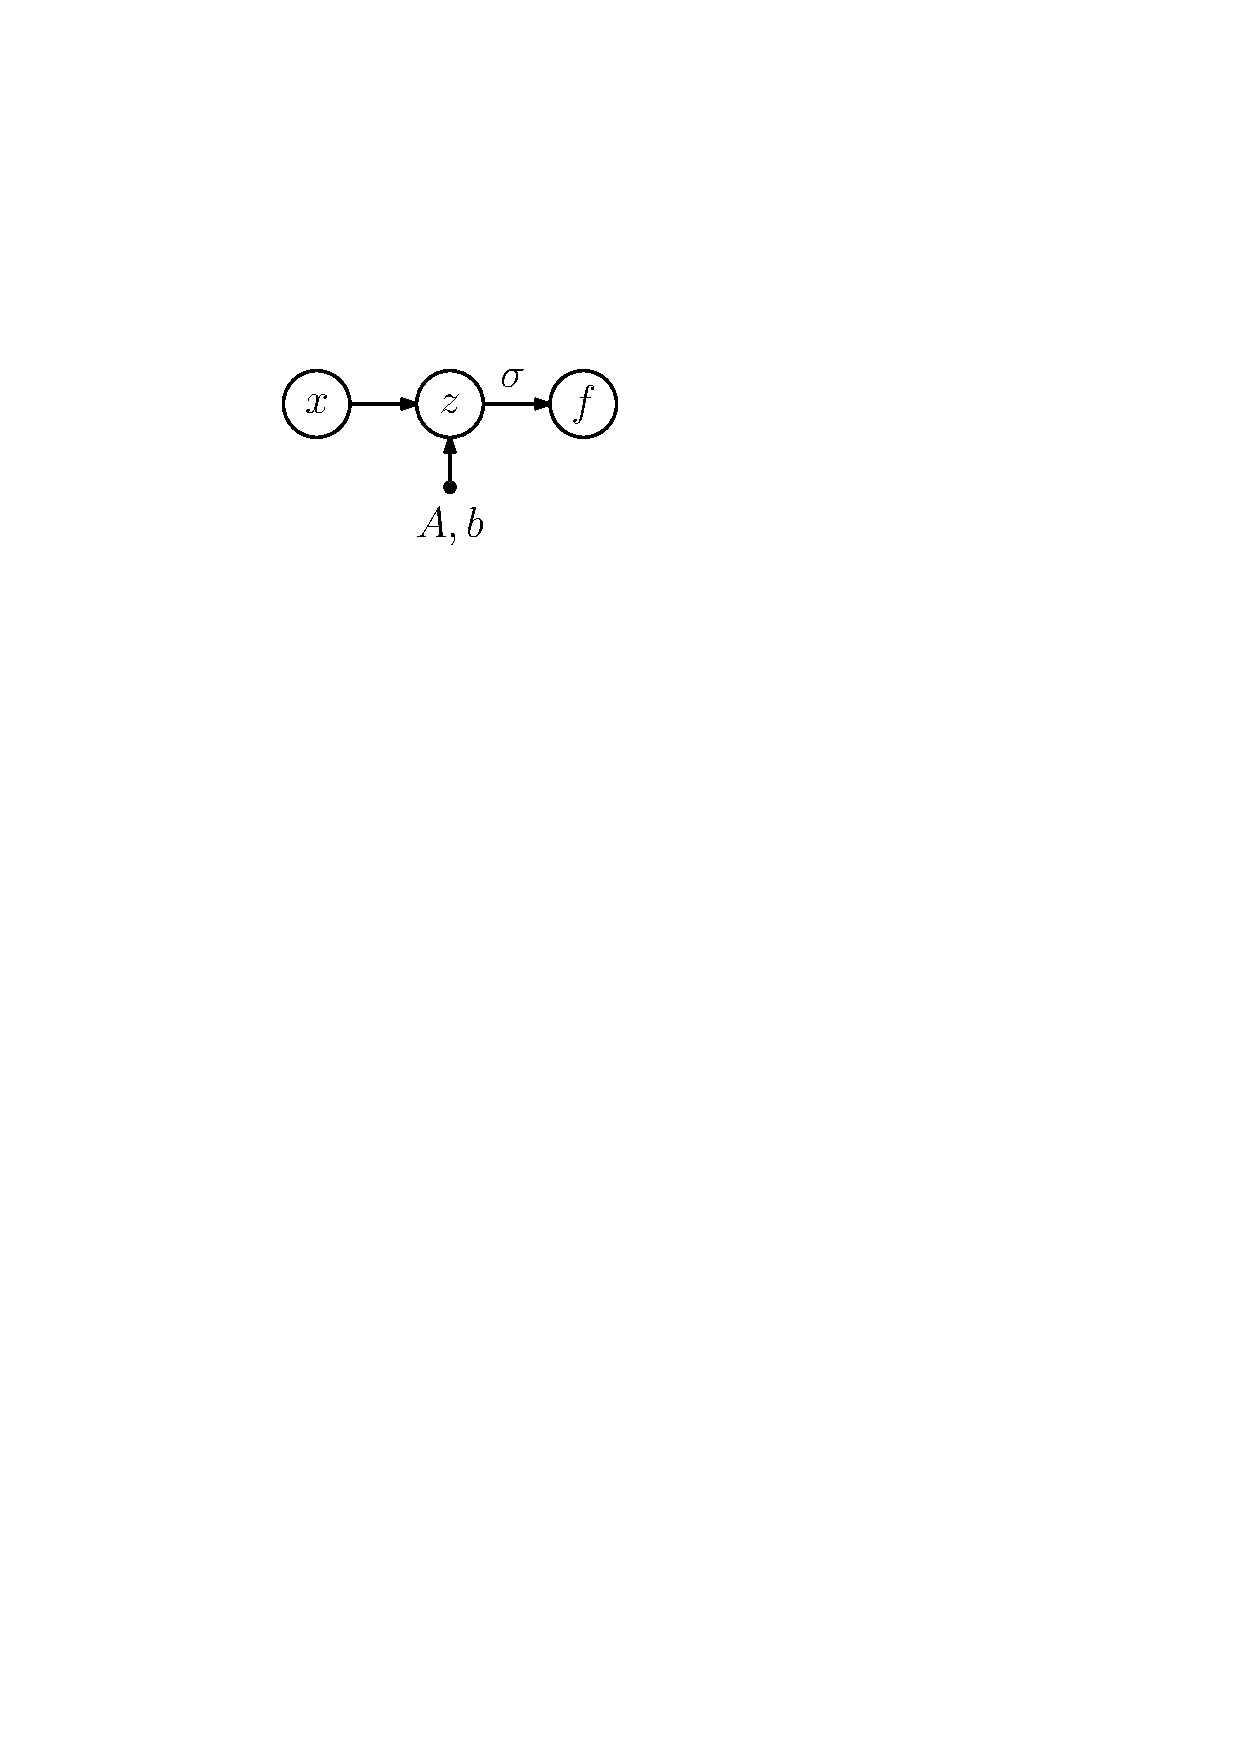
\includegraphics[width = 0.3\hsize]{./figures/network_z}
%   \end{figure}
  
%   \begin{align*}
%     \vec f &= \tanh(\underbrace{\mat A \vec x + \vec b}_{=:\vec z\in\R^M}) \in\R^M,\quad \vec x \in\R^N, \mat A \in\R^{M\times N}, \vec b\in\R^M
%   \end{align*}

% \end{frame}

% %%%%%%%%%%%%%%%%%%%%%%%%%%%%%%%%%%%%%%%%%
% \begin{frame}
%   \frametitle{Gradients of a Single-Layer Neural Network}
  
%   \begin{align*}
%     \vec f &= \tanh(\underbrace{\mat A \vec x + \vec b}_{=:\vec z\in\R^M}) \in\R^M,\quad \vec x \in\R^N, \mat A \in\R^{M\times N}, \vec b\in\R^M\\
%     \visible<1->{\frac{\partial \vec f}{\partial\vec b} &=} 
%     \visible<2->{\blue{\underbrace{\frac{\partial \vec
%     f}{\partial\vec z}}_{{M\times M}}} 
%      \red{\underbrace{\frac{\partial \vec z}{\partial \vec b}}_{{M\times M}}} \in\R^{M\times M}}
%     \visible<7->{\qquad\qquad\qquad \frac{\partial \vec f}{\partial\mat b}[i,j] = \sum_{l=1}^M \frac{\partial \vec f}{\partial\vec z}[i,l] \frac{\partial\vec z}{\partial \vec b}[l,j]}
%     \\
%     \visible<1->{\frac{\partial \vec f}{\partial \mat A} &=} 		
%     \visible<3->{\blue{\underbrace{\frac{\partial \vec
%     f}{\partial\vec z}}_{{M\times M}}} \orange{\underbrace{\frac{\partial
%     \vec z}{\partial \mat A}}_{{M\times (M\times N)}}}  \in\R^{M\times (M\times N)}
%     \qquad}
%     \visible<8->{\frac{\partial \vec f}{\partial\mat A}[i,j,k] = \sum_{l=1}^M \frac{\partial \vec f}{\partial\vec z}[i,l] \frac{\partial\vec z}{\partial \mat A}[l,j,k]}
%   \end{align*}
%   \vspace{-5mm}
%   \begin{align*}
%    \visible<4->{\blue{\frac{\partial\vec f}{\partial\vec z}} =\underbrace{\blue{\diag(1 - \tanh^2(\vec z))}}_{\in\:\R^{M\times M}}}
%    \quad
% 	\visible<5->{\red{\frac{\partial \vec z}{\partial \vec b}} =\underbrace{\red{\mat I}}_{\in\:\R^{M\times M}}}
% 	\quad
% 	\visible<6->{\orange{\frac{\partial \vec z}{\partial \mat A}} \quad =\underbrace{\orange{\scriptsize\begin{bmatrix}
% 	\vec x\T & \cdot & \vec 0\T & \cdot & \vec 0\T  \\
% 	\cdot & & \cdot & & \cdot  \\
% 	\vec 0\T & \cdot & \vec x\T & \cdot & \vec 0\T \\
% 	\cdot & & \cdot & & \cdot \\
% 	\vec 0\T & \cdot & \vec 0\T & \cdot & \vec x\T 
% 	\end{bmatrix}}}_{\in\:\R^{M \times (M \times N)}}}
%   \end{align*}

  
% \end{frame}

% % %%%%%%%%%%%%%%%%%%%%%%%%%%%%%%%%%%%%%%%%%
% % \begin{frame}

% % \begin{tt}
% %  \green{\small
% %  import numpy as np\\
% %  def NN(x, A, b):\\[1mm]  
% %  \qquad     M, N = A.shape\\
    
% %  \qquad     z = A.dot(x) + b\\
% %  \qquad     f = np.tanh(z)\\[1mm]
    
% %  \qquad     \# partial derivatives\\
% %  \qquad     dfdz = 1-f**2\\
    
% %  \qquad     dzdx = A\\
% %  \qquad     dzdb = np.eye(M)\\
% %  \qquad     dzdA = np.zeros((M, M, N))\\
    
% %  \qquad     for i in range(M):\\
% %  \qquad         \qquad dzdA[i,i,:] = x.T\\[1mm]
     
% %  \qquad     \# gradients\\
% %  \qquad     dfdx = np.einsum('il, lj', dfdz, dzdx)\\
% %  \qquad     dfdb = np.einsum('il, lj', dfdz, dzdb)\\
% %  \qquad     dfdA = np.einsum('il, ljk', dfdz, dzdA)\\[1mm]
% %  \qquad     return f, dfdA, dfdb, dfdx}
% %  \end{tt}
% %  \end{frame}
  

% %%%%%%%%%%%%%%%%%%%%%%%%%%%%%%%%%%%%%%%%%
% \begin{frame}
% \frametitle{Putting Things Together}
% \begin{itemize}[<+->]
%   \item Inputs $\vec x \in \R^N$
%   \item Observed outputs $\vec y = f_{\vec \theta}(\vec x) + \vec\epsilon \in \R^M \,, \vec \epsilon \sim\gauss{\vec 0}{\mat\Sigma}$
%   \item Train single-layer neural network with  
%   \begin{align*}
%     f_{\vec \theta}(\vec x) =  \tanh(\vec z(\vx)) \in \R^M\,,
%     \quad 
%     \vec z = \mat A\vec x + \vec b \in \R^M\,,
%     \quad 
%     \vec\theta = \{\mat A, \vec b\}
%   %  \\
%   %  \vec t &= \vec f_L
%   \end{align*}
%   \item Find $\vec A, \vec b$, such that
%     the squared loss
%     $$
%     L(\vec\theta) = \tfrac{1}{2}\|\vec e\|^2 \in \R\,,
%     \quad 
%     \vec e = \vec y - \vec f_{\vec \theta}(\vec z) \in \R^M
%     $$
%     is minimized
%   \end{itemize}
% \end{frame}

% \begin{frame}
% \frametitle{Putting Things Together}

% Partial derivatives:
%     \begin{align*}
%       \begin{array}{ll}
%         \displaystyle
%       \frac{\partial L}{\partial \mat A} &\displaystyle = \redish{\frac{\partial L}{\partial
%       \vec e}}\frac{\partial\vec e}{\partial \vec f}\blue{\frac{\partial \vec f}{\partial\vec
%         z}}\orange{\frac{\partial \vec z}{\partial \mat A}}\\
%         \displaystyle
%       \frac{\partial L}{\partial \vec b} &\displaystyle =  \redish{\frac{\partial L}{\partial
%       \vec e}}\frac{\partial\vec e}{\partial \vec f}\blue{\frac{\partial \vec f}{\partial\vec
%         z}}\red{\frac{\partial \vec z}{\partial \vec b}}
%       \end{array}
%     \end{align*}
    
%     \begin{align*}
%     \begin{array}{l}
%       \displaystyle                                        	  \redish{\frac{\partial L}{\partial
%       \vec e} = \underbrace{\vec e\T}_{\in\:\R^{1\times M}}}
%       \qquad
%       \frac{\partial \vec e}{\partial
%       \vec f} = \underbrace{-\vec I}_{\in\:\R^{M \times M}}
%       \qquad
%       \blue{\frac{\partial \vec
%       f}{\partial \mat z} = \underbrace{\diag(1 - \tanh^2(\vec z))}_{\in\:\R^{M\times M}}}
%       \\
%       \displaystyle
%       \orange{\frac{\partial \vec
%       z}{\partial \mat A} =
%       \underbrace{\begin{bmatrix}
% 	\vec x\T & \cdot & \vec 0\T & \cdot & \vec 0\T  \\
% 	\cdot & & \cdot & & \cdot  \\
% 	\vec 0\T & \cdot & \vec x\T & \cdot & \vec 0\T \\
% 	\cdot & & \cdot & & \cdot \\
% 	\vec 0\T & \cdot & \vec 0\T & \cdot & \vec x\T 
% 	\end{bmatrix}}_{\in\:\R^{M \times (M \times N)}}}
%       \qquad  
%       \red{\frac{\partial \vec
%       z}{\partial \mat b}  = \underbrace{\vec I}_{\in\:\R^{M \times M}}}
%     \end{array}
%     \end{align*}
% \end{frame}

% %\begin{frame}
 
% % \frametitle{Gradient descent for neural network optimisation}

% % \emph{Goal:} Find the local optimum of loss \(L_{\vec \theta^*} \in \R\) where \({\vec \theta}^* = \{\mat A^*, \vec b^* \}\) \\

% % Gradient descent algorithm:
% % \begin{enumerate}
% % \item Initialise neural network parameters, \({\vec \theta}_0\ = \{\mat A_0, \vec b_0 \}\)
% % \item Compute gradient of \(L\) w.r.t. parameters, \(\frac{\partial L}{\partial \vec \theta_0}\) 
% % \item Update initial guess \({\vec \theta}_0\) using chain rule:
% % \begin{align*}
% % {\vec \theta_{i+1}} = {\vec \theta_{i}} + \Delta{{\vec \theta}_i} =  {\vec \theta_{i}} - \gamma (\frac{\partial L}{\partial \vec \theta_i} (\vec \theta_i))\T
% % \end{align*}
% % \arrow Note: parameter update is the direction of steepest \emph{de}scent
% % \end{enumerate}

% % \visible<2>{
% % \vspace{2mm}
% % For suitable step-size \(\gamma\), the sequence \( L_{{\vec \theta}_0}(\vec x) \geq L_{{\vec \theta}_1}(\vec x) \geq \cdots\) converges to a local minimum \(L_{\vec \theta^*}(\vec x)\). }

% % \visible<1>{
% % 	\vspace{-1.3cm}
% % 	\begin{figure}
% %     \centering
% %     \includegraphics[width=0.45\hsize]{./figures/graddescent.eps}
% %   \end{figure}}



% % \end{frame}


% %%%%%%%%%%%%%%%%%%%%%%%%%%%%%%
% \begin{frame}
%   \frametitle{Gradients of a Multi-Layer Neural Network}
% \vspace{-8mm}
% \begin{equation}
% L(\vtheta_1, \vtheta_2,\vtheta_3) = ||\vy - \vec f_{\vtheta_3}(\vec f_{\vtheta_2}(\vec f_{\vtheta_1}(\vx)))||^2
% \end{equation}
% \vspace{-6mm}
% \begin{figure}
%     \centering
%     %\includegraphics[width = 0.8\hsize]{./figures/NN_forward}
%     \scalebox{0.5}{\tikzstyle{ipe stylesheet} = [
  ipe import,
  even odd rule,
  line join=round,
  line cap=butt,
  ipe pen normal/.style={line width=0.4},
  ipe pen heavier/.style={line width=0.8},
  ipe pen fat/.style={line width=1.2},
  ipe pen ultrafat/.style={line width=2},
  ipe pen normal,
  ipe mark normal/.style={ipe mark scale=3},
  ipe mark large/.style={ipe mark scale=5},
  ipe mark small/.style={ipe mark scale=2},
  ipe mark tiny/.style={ipe mark scale=1.1},
  ipe mark normal,
  /pgf/arrow keys/.cd,
  ipe arrow normal/.style={scale=7},
  ipe arrow large/.style={scale=10},
  ipe arrow small/.style={scale=5},
  ipe arrow tiny/.style={scale=3},
  ipe arrow normal,
  /tikz/.cd,
  ipe arrows, % update arrows
  <->/.tip = ipe normal,
  ipe dash normal/.style={dash pattern=},
  ipe dash dashed/.style={dash pattern=on 4bp off 4bp},
  ipe dash dotted/.style={dash pattern=on 1bp off 3bp},
  ipe dash dash dotted/.style={dash pattern=on 4bp off 2bp on 1bp off 2bp},
  ipe dash dash dot dotted/.style={dash pattern=on 4bp off 2bp on 1bp off 2bp on 1bp off 2bp},
  ipe dash normal,
  ipe node/.append style={font=\normalsize},
  ipe stretch normal/.style={ipe node stretch=1},
  ipe stretch normal,
  ipe opacity 10/.style={opacity=0.1},
  ipe opacity 30/.style={opacity=0.3},
  ipe opacity 50/.style={opacity=0.5},
  ipe opacity 75/.style={opacity=0.75},
  ipe opacity opaque/.style={opacity=1},
  ipe opacity opaque,
]
\definecolor{red}{rgb}{1,0,0}%
\definecolor{green}{rgb}{0,1,0}%
\definecolor{blue}{rgb}{0,0,1}%
\definecolor{yellow}{rgb}{1,1,0}%
\definecolor{orange}{rgb}{1,0.647,0}%
\definecolor{gold}{rgb}{1,0.843,0}%
\definecolor{purple}{rgb}{0.627,0.125,0.941}%
\definecolor{gray}{rgb}{0.745,0.745,0.745}%
\definecolor{brown}{rgb}{0.647,0.165,0.165}%
\definecolor{navy}{rgb}{0,0,0.502}%
\definecolor{pink}{rgb}{1,0.753,0.796}%
\definecolor{seagreen}{rgb}{0.18,0.545,0.341}%
\definecolor{turquoise}{rgb}{0.251,0.878,0.816}%
\definecolor{violet}{rgb}{0.933,0.51,0.933}%
\definecolor{darkblue}{rgb}{0,0,0.545}%
\definecolor{darkcyan}{rgb}{0,0.545,0.545}%
\definecolor{darkgray}{rgb}{0.663,0.663,0.663}%
\definecolor{darkgreen}{rgb}{0,0.392,0}%
\definecolor{darkmagenta}{rgb}{0.545,0,0.545}%
\definecolor{darkorange}{rgb}{1,0.549,0}%
\definecolor{darkred}{rgb}{0.545,0,0}%
\definecolor{lightblue}{rgb}{0.678,0.847,0.902}%
\definecolor{lightcyan}{rgb}{0.878,1,1}%
\definecolor{lightgray}{rgb}{0.827,0.827,0.827}%
\definecolor{lightgreen}{rgb}{0.565,0.933,0.565}%%
\definecolor{lightyellow}{rgb}{1,1,0.878}%
\definecolor{black}{rgb}{0,0,0}%
\definecolor{white}{rgb}{1,1,1}%
\begin{tikzpicture}[ipe stylesheet]
  \draw[ipe pen fat]
    (144, 768) rectangle (160, 704);
  \draw[ipe pen fat]
    (256, 768) rectangle (272, 704);
  \draw[ipe pen fat]
    (432, 768) rectangle (448, 704);
  \draw[ipe pen fat]
    (96, 736) circle[radius=16];
  \draw[ipe pen fat]
    (496, 736) circle[radius=16];
  \draw[ipe pen fat, ->]
    (112, 736)
     -- (144, 736);
  \draw[ipe pen fat, ipe dash dashed, ->]
    (272, 736)
     -- (320, 736);
  \draw[ipe pen fat, ->]
    (448, 736)
     -- (480, 736);
  \node[ipe node, font=\Large]
     at (91.741, 732.812) {$\vec{x}$};
  \node[ipe node, font=\Large]
     at (488.698, 732.093) {$\vec{f}_K$};
  \node[ipe node, font=\Large]
     at (135, 664) {$\vec{A}_0, \vec{b}_0$};
  \node[ipe node, font=\Large]
     at (408, 664) {$\vec{A}_{K}, \vec{b}_{K}$};
  \draw[ipe pen fat]
    (560, 736) circle[radius=16];
  \draw[ipe pen fat, ->]
    (512, 736)
     -- (544, 736);
  \node[ipe node, font=\Large]
     at (555.221, 731.099) {$L$};
  \draw[ipe pen fat]
    (320, 768) rectangle (336, 704);
  \draw[ipe pen fat]
    (384, 736) circle[radius=16];
  \draw[ipe pen fat, ->]
    (336, 736)
     -- (368, 736);
  \node[ipe node, font=\Large]
     at (371, 732.508) {$\vec{f}_{K-1}$};
  \draw[ipe pen fat, ->]
    (400, 736)
     -- (432, 736);
  \node[ipe node, font=\Large]
     at (297, 664) {$\vec{A}_{K-1}, \vec{b}_{K-1}$};
  \draw[ipe pen fat, ->]
    (152, 680)
     -- (152, 704);
  \draw[ipe pen fat, ->]
    (264, 680)
     -- (264, 704);
  \draw[ipe pen fat, ->]
    (328, 680)
     -- (328, 704);
  \draw[ipe pen fat, ->]
    (440, 680)
     -- (440, 704);
  \draw[ipe pen fat]
    (208, 736) circle[radius=16];
  \draw[ipe pen fat, ->]
    (160, 736)
     -- (192, 736);
  \node[ipe node, font=\Large]
     at (202.794, 732.093) {$\vec{f}_1$};
  \draw[ipe pen fat, ->]
    (224, 736)
     -- (256, 736);
  \node[ipe node, font=\Large]
     at (247, 664) {$\vec{A}_1, \vec{b}_1$};
\end{tikzpicture}

%%% Local Variables:
%%% mode: latex
%%% TeX-master: "../mml-book"
%%% End:
}
%   \end{figure}
  
%   \begin{itemize}
%   \item Inputs $\vec x$, observed outputs $\vec y$
%   \item Train multi-layer neural network with  
%   \begin{align*}
%     \vec f_0 &= \vec x\\
%     \vec f_i &= \sigma_i(\mat A_{i-1}\vec f_{i-1} + \vec b_{i-1})\,,
%                \quad i = 1,\dotsc, K
%   \end{align*}
%   \vspace{-5mm}
%   \pause
%   \item Find $\vec A_j, \vec b_j$ for $j = 0,\dotsc, K-1$, such that
%     the squared loss
%     $$
%     L(\vec\theta) = \|\vec y - \vec f_{K,\vec \theta}( \vec x)\|^2
%     $$
%     is minimized, where $
%       \vec\theta = \{\mat A_j, \vec b_j\}\,,\quad j = 0, \dotsc, K-1
%     $
%   \end{itemize}

  
  
% \end{frame}


% %%%%%%%%%%%%%%%%%%%%%%%%%%%%%%%%%%%%%%%%%
% \begin{frame}
%   \frametitle{Gradients of a Multi-Layer Neural Network}
% \vspace{-8mm}
% \begin{equation}
% L(\vtheta_1, \vtheta_2,\vtheta_3) = ||\vy - \vec f_{\vtheta_3}(\vec f_{\vtheta_2}(\vec f_{\vtheta_1}(\vx)))||^2
% \end{equation}
% \vspace{-6mm}
%   \onslide*<1>{
%   \begin{figure}
%     \centering
%     % \includegraphics[width = 0.7\hsize]{./figures/NN1}
%      \scalebox{0.5}{\tikzstyle{ipe stylesheet} = [
  ipe import,
  even odd rule,
  line join=round,
  line cap=butt,
  ipe pen normal/.style={line width=0.4},
  ipe pen heavier/.style={line width=0.8},
  ipe pen fat/.style={line width=1.2},
  ipe pen ultrafat/.style={line width=2},
  ipe pen normal,
  ipe mark normal/.style={ipe mark scale=3},
  ipe mark large/.style={ipe mark scale=5},
  ipe mark small/.style={ipe mark scale=2},
  ipe mark tiny/.style={ipe mark scale=1.1},
  ipe mark normal,
  /pgf/arrow keys/.cd,
  ipe arrow normal/.style={scale=7},
  ipe arrow large/.style={scale=10},
  ipe arrow small/.style={scale=5},
  ipe arrow tiny/.style={scale=3},
  ipe arrow normal,
  /tikz/.cd,
  ipe arrows, % update arrows
  <->/.tip = ipe normal,
  ipe dash normal/.style={dash pattern=},
  ipe dash dashed/.style={dash pattern=on 4bp off 4bp},
  ipe dash dotted/.style={dash pattern=on 1bp off 3bp},
  ipe dash dash dotted/.style={dash pattern=on 4bp off 2bp on 1bp off 2bp},
  ipe dash dash dot dotted/.style={dash pattern=on 4bp off 2bp on 1bp off 2bp on 1bp off 2bp},
  ipe dash normal,
  ipe node/.append style={font=\normalsize},
  ipe stretch normal/.style={ipe node stretch=1},
  ipe stretch normal,
  ipe opacity 10/.style={opacity=0.1},
  ipe opacity 30/.style={opacity=0.3},
  ipe opacity 50/.style={opacity=0.5},
  ipe opacity 75/.style={opacity=0.75},
  ipe opacity opaque/.style={opacity=1},
  ipe opacity opaque,
]
\definecolor{red}{rgb}{1,0,0}%
\definecolor{green}{rgb}{0,1,0}%
\definecolor{blue}{rgb}{0,0,1}%
\definecolor{yellow}{rgb}{1,1,0}%
\definecolor{orange}{rgb}{1,0.647,0}%
\definecolor{gold}{rgb}{1,0.843,0}%
\definecolor{purple}{rgb}{0.627,0.125,0.941}%
\definecolor{gray}{rgb}{0.745,0.745,0.745}%
\definecolor{brown}{rgb}{0.647,0.165,0.165}%
\definecolor{navy}{rgb}{0,0,0.502}%
\definecolor{pink}{rgb}{1,0.753,0.796}%
\definecolor{seagreen}{rgb}{0.18,0.545,0.341}%
\definecolor{turquoise}{rgb}{0.251,0.878,0.816}%
\definecolor{violet}{rgb}{0.933,0.51,0.933}%
\definecolor{darkblue}{rgb}{0,0,0.545}%
\definecolor{darkcyan}{rgb}{0,0.545,0.545}%
\definecolor{darkgray}{rgb}{0.663,0.663,0.663}%
\definecolor{darkgreen}{rgb}{0,0.392,0}%
\definecolor{darkmagenta}{rgb}{0.545,0,0.545}%
\definecolor{darkorange}{rgb}{1,0.549,0}%
\definecolor{darkred}{rgb}{0.545,0,0}%
\definecolor{lightblue}{rgb}{0.678,0.847,0.902}%
\definecolor{lightcyan}{rgb}{0.878,1,1}%
\definecolor{lightgray}{rgb}{0.827,0.827,0.827}%
\definecolor{lightgreen}{rgb}{0.565,0.933,0.565}%%
\definecolor{lightyellow}{rgb}{1,1,0.878}%
\definecolor{black}{rgb}{0,0,0}%
\definecolor{white}{rgb}{1,1,1}%
\begin{tikzpicture}[ipe stylesheet]
  \draw[ipe pen fat, white]
    (144, 768) rectangle (160, 704);
  \draw[ipe pen fat, white]
    (256, 768) rectangle (272, 704);
  \draw[ipe pen fat]
    (432, 768) rectangle (448, 704);
  \draw[white, ipe pen fat]
    (96, 736) circle[radius=16];
  \draw[ipe pen fat]
    (496, 736) circle[radius=16];
  \draw[white, ipe pen fat, <-]
    (112, 736)
     -- (144, 736);
  \draw[white, ipe pen fat, ipe dash dashed, <-]
    (272, 736)
     -- (320, 736);
  \draw[red, ipe pen fat, <-]
    (448, 736)
     -- (480, 736);
  \node[ipe node, font=\Large, text=white]
     at (91.741, 732.812) {$\vec{x}$};
  \node[ipe node, font=\Large]
     at (488.698, 734) {$\vec{f}_K$};
  \node[ipe node, font=\Large, text=white]
     at (135, 664) {$\vec{A}_1, \vec{b}_1$};
  \node[ipe node, font=\Large]
     at (408, 664) {$\vec{A}_{K}, \vec{b}_{K}$};
  \draw[ipe pen fat]
    (560, 736) circle[radius=16];
  \draw[red, ipe pen fat, <-]
    (512, 736)
     -- (544, 736);
  \node[ipe node, font=\Large]
     at (555.221, 731.099) {$L$};
  \draw[white, ipe pen fat]
    (320, 768) rectangle (336, 704);
  \draw[white, ipe pen fat]
    (384, 736) circle[radius=16];
  \draw[white, ipe pen fat, <-]
    (336, 736)
     -- (368, 736);
  \node[ipe node, font=\Large, text=white]
     at (371, 734) {$\vec{f}_{K-1}$};
  \draw[white, ipe pen fat, <-]
    (400, 736)
     -- (432, 736);
  \node[ipe node, font=\Large, text=white]
     at (297, 664) {$\vec{A}_{K-1}, \vec{b}_{K-1}$};
  \draw[white, ipe pen fat, ->]
    (152, 680)
     -- (152, 704);
  \draw[white, ipe pen fat, ->]
    (264, 680)
     -- (264, 704);
  \draw[white, ipe pen fat, ->]
    (328, 680)
     -- (328, 704);
  \draw[ipe pen fat, ->]
    (440, 680)
     -- (440, 704);
  \draw[white, ipe pen fat]
    (208, 736) circle[radius=16];
  \draw[white, ipe pen fat, <-]
    (160, 736)
     -- (192, 736);
  \node[ipe node, font=\Large, text=white]
     at (202.794, 734) {$\vec{f}_1$};
  \draw[white, ipe pen fat, <-]
    (224, 736)
     -- (256, 736);
  \node[ipe node, font=\Large, text=white]
     at (247, 664) {$\vec{A}_2, \vec{b}_2$};
\end{tikzpicture}


%%% Local Variables:
%%% mode: latex
%%% TeX-master: "../lecture_vector_calculus"
%%% End:
}
%   \end{figure}
% }
% \onslide*<2>{
%   \begin{figure}
%     \centering
% %    \includegraphics[width = 0.7\hsize]{./figures/NN2}
%     \scalebox{0.5}{\tikzstyle{ipe stylesheet} = [
  ipe import,
  even odd rule,
  line join=round,
  line cap=butt,
  ipe pen normal/.style={line width=0.4},
  ipe pen heavier/.style={line width=0.8},
  ipe pen fat/.style={line width=1.2},
  ipe pen ultrafat/.style={line width=2},
  ipe pen normal,
  ipe mark normal/.style={ipe mark scale=3},
  ipe mark large/.style={ipe mark scale=5},
  ipe mark small/.style={ipe mark scale=2},
  ipe mark tiny/.style={ipe mark scale=1.1},
  ipe mark normal,
  /pgf/arrow keys/.cd,
  ipe arrow normal/.style={scale=7},
  ipe arrow large/.style={scale=10},
  ipe arrow small/.style={scale=5},
  ipe arrow tiny/.style={scale=3},
  ipe arrow normal,
  /tikz/.cd,
  ipe arrows, % update arrows
  <->/.tip = ipe normal,
  ipe dash normal/.style={dash pattern=},
  ipe dash dashed/.style={dash pattern=on 4bp off 4bp},
  ipe dash dotted/.style={dash pattern=on 1bp off 3bp},
  ipe dash dash dotted/.style={dash pattern=on 4bp off 2bp on 1bp off 2bp},
  ipe dash dash dot dotted/.style={dash pattern=on 4bp off 2bp on 1bp off 2bp on 1bp off 2bp},
  ipe dash normal,
  ipe node/.append style={font=\normalsize},
  ipe stretch normal/.style={ipe node stretch=1},
  ipe stretch normal,
  ipe opacity 10/.style={opacity=0.1},
  ipe opacity 30/.style={opacity=0.3},
  ipe opacity 50/.style={opacity=0.5},
  ipe opacity 75/.style={opacity=0.75},
  ipe opacity opaque/.style={opacity=1},
  ipe opacity opaque,
]
\definecolor{red}{rgb}{1,0,0}%
\definecolor{green}{rgb}{0,1,0}%
\definecolor{blue}{rgb}{0,0,1}%
\definecolor{yellow}{rgb}{1,1,0}%
\definecolor{orange}{rgb}{1,0.647,0}%
\definecolor{gold}{rgb}{1,0.843,0}%
\definecolor{purple}{rgb}{0.627,0.125,0.941}%
\definecolor{gray}{rgb}{0.745,0.745,0.745}%
\definecolor{brown}{rgb}{0.647,0.165,0.165}%
\definecolor{navy}{rgb}{0,0,0.502}%
\definecolor{pink}{rgb}{1,0.753,0.796}%
\definecolor{seagreen}{rgb}{0.18,0.545,0.341}%
\definecolor{turquoise}{rgb}{0.251,0.878,0.816}%
\definecolor{violet}{rgb}{0.933,0.51,0.933}%
\definecolor{darkblue}{rgb}{0,0,0.545}%
\definecolor{darkcyan}{rgb}{0,0.545,0.545}%
\definecolor{darkgray}{rgb}{0.663,0.663,0.663}%
\definecolor{darkgreen}{rgb}{0,0.392,0}%
\definecolor{darkmagenta}{rgb}{0.545,0,0.545}%
\definecolor{darkorange}{rgb}{1,0.549,0}%
\definecolor{darkred}{rgb}{0.545,0,0}%
\definecolor{lightblue}{rgb}{0.678,0.847,0.902}%
\definecolor{lightcyan}{rgb}{0.878,1,1}%
\definecolor{lightgray}{rgb}{0.827,0.827,0.827}%
\definecolor{lightgreen}{rgb}{0.565,0.933,0.565}%%
\definecolor{lightyellow}{rgb}{1,1,0.878}%
\definecolor{black}{rgb}{0,0,0}%
\definecolor{white}{rgb}{1,1,1}%
\begin{tikzpicture}[ipe stylesheet]
  \draw[ipe pen fat, white]
    (144, 768) rectangle (160, 704);
  \draw[ipe pen fat, white]
    (256, 768) rectangle (272, 704);
  \draw[ipe pen fat]
    (432, 768) rectangle (448, 704);
  \draw[white, ipe pen fat]
    (96, 736) circle[radius=16];
  \draw[ipe pen fat]
    (496, 736) circle[radius=16];
  \draw[white, ipe pen fat, <-]
    (112, 736)
     -- (144, 736);
  \draw[white, ipe pen fat, ipe dash dashed, <-]
    (272, 736)
     -- (320, 736);
  \draw[red, ipe pen fat, <-]
    (448, 736)
     -- (480, 736);
  \node[ipe node, font=\Large, text=white]
     at (91.741, 732.812) {$\vec{x}$};
  \node[ipe node, font=\Large]
     at (488.698, 734) {$\vec{f}_K$};
  \node[ipe node, font=\Large, text=white]
     at (135, 664) {$\vec{A}_1, \vec{b}_1$};
  \node[ipe node, font=\Large]
     at (408, 664) {$\vec{A}_{K}, \vec{b}_{K}$};
  \draw[ipe pen fat]
    (560, 736) circle[radius=16];
  \draw[red, ipe pen fat, <-]
    (512, 736)
     -- (544, 736);
  \node[ipe node, font=\Large]
     at (555.221, 731.099) {$L$};
  \draw[ipe pen fat]
    (320, 768) rectangle (336, 704);
  \draw[ipe pen fat]
    (384, 736) circle[radius=16];
  \draw[red, ipe pen fat, <-]
    (336, 736)
     -- (368, 736);
  \node[ipe node, font=\Large]
     at (371, 734) {$\vec{f}_{K-1}$};
  \draw[red, ipe pen fat, <-]
    (400, 736)
     -- (432, 736);
  \node[ipe node, font=\Large]
     at (297, 664) {$\vec{A}_{K-1}, \vec{b}_{K-1}$};
  \draw[white, ipe pen fat, ->]
    (152, 680)
     -- (152, 704);
  \draw[white, ipe pen fat, ->]
    (264, 680)
     -- (264, 704);
  \draw[ ipe pen fat, ->]
    (328, 680)
     -- (328, 704);
  \draw[ipe pen fat, ->]
    (440, 680)
     -- (440, 704);
  \draw[white, ipe pen fat]
    (208, 736) circle[radius=16];
  \draw[white, ipe pen fat, <-]
    (160, 736)
     -- (192, 736);
  \node[ipe node, font=\Large, text=white]
     at (202.794, 734) {$\vec{f}_1$};
  \draw[white, ipe pen fat, <-]
    (224, 736)
     -- (256, 736);
  \node[ipe node, font=\Large, text=white]
     at (247, 664) {$\vec{A}_2, \vec{b}_2$};
\end{tikzpicture}



% \begin{tikzpicture}[ipe stylesheet]
%   \draw[white, ipe pen fat]
%     (144, 768) rectangle (160, 704);
%   \draw[white, ipe pen fat]
%     (256, 768) rectangle (272, 704);
%   \draw[ipe pen fat]
%     (432, 768) rectangle (448, 704);
%   \draw[white, ipe pen fat]
%     (96, 736) circle[radius=16];
%   \draw[ipe pen fat]
%     (496, 736) circle[radius=16];
%   \draw[white, ipe pen fat, ->]
%     (112, 736)
%      -- (144, 736);
%   \draw[white, ipe pen fat, ipe dash dashed, ->]
%     (272, 728)
%      -- (320, 728);
%   \draw[ipe pen fat, ->]
%     (448, 728)
%      -- (480, 728);
%   \node[ipe node, font=\Large, text=white]
%      at (92.009, 732.912) {$\vec x$};
%   \node[ipe node, font=\Large]
%      at (488.899, 732.414) {$\vec f_K$};
%   \node[ipe node, font=\Large, text=white]
%      at (135.123, 664) {$\vec A_1, \vec b_1$};
%   \node[ipe node, font=\Large]
%      at (408.594, 664) {$\mat A_{K-1}, \vec b_{K-1}$};
%   \draw[red, ipe pen fat, ->]
%     (480, 744)
%      -- (448, 744);
%   \draw[white, ipe pen fat, ipe dash dashed, ->]
%     (320, 744)
%      -- (272, 744);
%   \draw[ipe pen fat]
%     (560, 736) circle[radius=16];
%   \draw[ipe pen fat, ->]
%     (512, 728)
%      -- (544, 728);
%   \draw[red, ipe pen fat, ->]
%     (544, 744)
%      -- (512, 744);
%   \node[ipe node, font=\Large]
%      at (555.221, 731.099) {$L$};
%   \draw[ipe pen fat]
%     (320, 768) rectangle (336, 704);
%   \draw[ipe pen fat]
%     (384, 736) circle[radius=16];
%   \draw[ipe pen fat, ->]
%     (336, 728)
%      -- (368, 728);
%   \node[ipe node, font=\Large]
%      at (370.534, 732.508) {$\vec f_{K-1}$};
%   \draw[red, ipe pen fat, ->]
%     (368, 744)
%      -- (336, 744);
%   \draw[ipe pen fat, ->]
%     (400, 728)
%      -- (432, 728);
%   \draw[red, ipe pen fat, ->]
%     (432, 744)
%      -- (400, 744);
%   \node[ipe node, font=\Large]
%      at (296.594, 664) {$\mat A_{K-2}, \vec b_{K-2}$};
%   \draw[white, ipe pen fat, ->]
%     (152, 680)
%      -- (152, 704);
%   \draw[white, ipe pen fat, ->]
%     (264, 680)
%      -- (264, 704);
%   \draw[ipe pen fat, ->]
%     (328, 680)
%      -- (328, 704);
%   \draw[ipe pen fat, ->]
%     (440, 680)
%      -- (440, 704);
%   \pic[ipe mark large, white]
%      at (152, 680) {ipe disk};
%   \pic[ipe mark large, white]
%      at (264, 680) {ipe disk};
%   \pic[ipe mark large]
%      at (328, 680) {ipe disk};
%   \pic[ipe mark large]
%      at (440, 680) {ipe disk};
%   \draw[white, ipe pen fat]
%     (208, 736) circle[radius=16];
%   \draw[white, ipe pen fat, ->]
%     (160, 728)
%      -- (192, 728);
%   \node[ipe node, font=\Large, text=white]
%      at (200.899, 732.414) {$f_1$};
%   \draw[white, ipe pen fat, ->]
%     (192, 744)
%      -- (160, 744);
%   \draw[white, ipe pen fat, ->]
%     (224, 728)
%      -- (256, 728);
%   \draw[white, ipe pen fat, ->]
%     (256, 744)
%      -- (224, 744);
%   \node[ipe node, font=\Large, text=white]
%      at (247.123, 664) {$A_2, b_2$};
% \end{tikzpicture}

%%% Local Variables:
%%% mode: latex
%%% TeX-master: "../lecture_vector_calculus"
%%% End:
}
%   \end{figure}
% }
% \onslide*<3->{
%  \begin{figure}
%    \centering
%   \scalebox{0.5}{\tikzstyle{ipe stylesheet} = [
  ipe import,
  even odd rule,
  line join=round,
  line cap=butt,
  ipe pen normal/.style={line width=0.4},
  ipe pen heavier/.style={line width=0.8},
  ipe pen fat/.style={line width=1.2},
  ipe pen ultrafat/.style={line width=2},
  ipe pen normal,
  ipe mark normal/.style={ipe mark scale=3},
  ipe mark large/.style={ipe mark scale=5},
  ipe mark small/.style={ipe mark scale=2},
  ipe mark tiny/.style={ipe mark scale=1.1},
  ipe mark normal,
  /pgf/arrow keys/.cd,
  ipe arrow normal/.style={scale=7},
  ipe arrow large/.style={scale=10},
  ipe arrow small/.style={scale=5},
  ipe arrow tiny/.style={scale=3},
  ipe arrow normal,
  /tikz/.cd,
  ipe arrows, % update arrows
  <->/.tip = ipe normal,
  ipe dash normal/.style={dash pattern=},
  ipe dash dashed/.style={dash pattern=on 4bp off 4bp},
  ipe dash dotted/.style={dash pattern=on 1bp off 3bp},
  ipe dash dash dotted/.style={dash pattern=on 4bp off 2bp on 1bp off 2bp},
  ipe dash dash dot dotted/.style={dash pattern=on 4bp off 2bp on 1bp off 2bp on 1bp off 2bp},
  ipe dash normal,
  ipe node/.append style={font=\normalsize},
  ipe stretch normal/.style={ipe node stretch=1},
  ipe stretch normal,
  ipe opacity 10/.style={opacity=0.1},
  ipe opacity 30/.style={opacity=0.3},
  ipe opacity 50/.style={opacity=0.5},
  ipe opacity 75/.style={opacity=0.75},
  ipe opacity opaque/.style={opacity=1},
  ipe opacity opaque,
]
\definecolor{red}{rgb}{1,0,0}%
\definecolor{black}{rgb}{0,0,0}%
\definecolor{white}{rgb}{1,1,1}%
\begin{tikzpicture}[ipe stylesheet]
  \draw[ipe pen fat]
    (144, 768) rectangle (160, 704);
  \draw[ipe pen fat]
    (256, 768) rectangle (272, 704);
  \draw[ipe pen fat]
    (432, 768) rectangle (448, 704);
  \draw[ipe pen fat]
    (96, 736) circle[radius=16];
  \draw[ipe pen fat]
    (496, 736) circle[radius=16];
  \draw[red, ipe pen fat, <-]
    (112, 736)
     -- (144, 736);
  \draw[red, ipe pen fat, ipe dash dashed, <-]
    (272, 736)
     -- (320, 736);
  \draw[red, ipe pen fat, <-]
    (448, 736)
     -- (480, 736);
  \node[ipe node, font=\Large]
     at (91.741, 734) {$\vec{x}$};
  \node[ipe node, font=\Large]
     at (488.698, 734) {$\vec{f}_K$};
  \node[ipe node, font=\Large]
     at (135, 664) {$\vec{A}_1, \vec{b}_1$};
  \node[ipe node, font=\Large]
     at (408, 664) {$\vec{A}_{K}, \vec{b}_{K}$};
  \draw[ipe pen fat]
    (560, 736) circle[radius=16];
  \draw[red, ipe pen fat, <-]
    (512, 736)
     -- (544, 736);
  \node[ipe node, font=\Large]
     at (555.221, 731.099) {$L$};
  \draw[ipe pen fat]
    (320, 768) rectangle (336, 704);
  \draw[ipe pen fat]
    (384, 736) circle[radius=16];
  \draw[red, ipe pen fat, <-]
    (336, 736)
     -- (368, 736);
  \node[ipe node, font=\Large]
     at (371, 734) {$\vec{f}_{K-1}$};
  \draw[red, ipe pen fat, <-]
    (400, 736)
     -- (432, 736);
  \node[ipe node, font=\Large]
     at (297, 664) {$\vec{A}_{K-1}, \vec{b}_{K-1}$};
  \draw[ipe pen fat, ->]
    (152, 680)
     -- (152, 704);
  \draw[ipe pen fat, ->]
    (264, 680)
     -- (264, 704);
  \draw[ipe pen fat, ->]
    (328, 680)
     -- (328, 704);
  \draw[ipe pen fat, ->]
    (440, 680)
     -- (440, 704);
  \draw[ipe pen fat]
    (208, 736) circle[radius=16];
  \draw[red, ipe pen fat, <-]
    (160, 736)
     -- (192, 736);
  \node[ipe node, font=\Large]
     at (202.794, 734) {$\vec{f}_1$};
  \draw[red, ipe pen fat, <-]
    (224, 736)
     -- (256, 736);
  \node[ipe node, font=\Large]
     at (247, 664) {$\vec{A}_2, \vec{b}_2$};
\end{tikzpicture}

%%% Local Variables:
%%% mode: latex
%%% TeX-master: "../lecture_vector_calculus"
%%% End:
}
%  \end{figure}
% }
% \vspace{-3mm}
%   \begin{align*}
%  \onslide+<1->{   \frac{\partial L}{\partial\vec\theta_{K}} &= \orange{\frac{\partial L}{\partial \vec f_K}}\blue{\frac{\partial \vec f_K}{\partial \vec\theta_{K}}}\\
% }
%     \onslide+<2->{    \frac{\partial L}{\partial\vec\theta_{K-1}} &=\orange{\frac{\partial
%                                                                     L}{\partial \vec f_K}}
%                                                                     \boxed{ \green{\frac{\partial \vec f_K}{\partial
%                                                                     \vec f_{K-1}}}
%                                                                     \blue{\frac{\partial\vec
%                                                                     f_{K-1}}{\partial \vec\theta_{K-1}}}}\\}
%     \onslide+<3->{    \frac{\partial L}{\partial\vec\theta_{K-2}} &=\orange{\frac{\partial
%                                                                     L}{\partial \vec f_K}}
%                                                                     \green{\frac{\partial \vec f_K}{\partial
%                                                                     \vec f_{K-1}}} \boxed{\green{\frac{\partial \vec f_{K-1}}{\partial
%                                                                     \vec f_{K-2}}}
%                                                                     \blue{\frac{\partial\vec
%                                                                     f_{K-2}}{\partial \vec\theta_{K-2}}}}\\}
%     \onslide+<4->{    \frac{\partial L}{\partial\vec\theta_{i}} &=\orange{\frac{\partial
%                                                                   L}{\partial \vec f_K}}
%                                                                   \green{\frac{\partial \vec f_K}{\partial
%                                                                   \vec f_{K-1}}\cdots}\boxed{\green{\frac{\partial \vec f_{i+1}}{\partial
%                                                                   \vec f_{i}}}
%                                                                   \blue{\frac{\partial\vec
%                                                                   f_{i}}{\partial
%                                                                   \vec\theta_{i}}}}
%                                                                   }
%   \end{align*}
% \onslide+<5>{\arrow Intermediate derivatives are stored during the forward pass}

%   % \begin{align*}
%   %   \frac{\partial \vec f_j}{\partial\vec f_{j-1}} = \mat A_{j-1}
%   % \end{align*}
% \end{frame}



% % %%%%%%%%%%%%%%%%%%%%%%%%%%%%%%%%%%%%%%%%%%%%%%%%%%%%%%
% %   \begin{frame}
% %     \frametitle{Example: Regression with Neural Networks}

% %     \begin{itemize}
% %     \item Linear regression with a neural network parametrized by \(\vec \theta, f_{\vec \theta}\):
% %       \begin{align*}
% %         y &= f_{\vec \theta}(\vec x) + \epsilon\,,\quad \epsilon \sim \gauss{0}{\sigma_\epsilon^2}
% %       \end{align*}
% %       \pause
% %     \item Given inputs $\vec x_n$ and corresponding (noisy)
% %       observations $y_n$, $n=1,\dotsc, N$, find parameters
% %       $\vec \theta^*$ that minimize the squared loss
% %         $$
% %         L(\vec\theta) = \sum_{n=1}^N (y_n - f_{\vec \theta}(\vec x_n))^2 =
% %         \norm{\vec y - \vec f(\mat X)}^2
% %         $$
% %   \end{itemize}
    
    
% %  \end{frame}




% %%% Local Variables:
% %%% mode: latex
% %%% TeX-master: "lecture_vector_calculus"
% %%% End:

% % %%%%%%%%%%%%%%%%%%%%%%%%%%%%%%%%%%%%%%%%%%%%%%%%%%%%%%
% % \begin{frame}
% %   \frametitle{Training Neural Networks as Maximum Likelihood Estimation}
% %   \begin{itemize}
% %   \item Training a neural network in the above way corresponds to
% %     \cemph{maximum likelihood estimation:}
% %       \begin{itemize}
% %         \item If $\vec y = NN(\vec x, \vec\theta) + \vec\epsilon,
% %           \quad \vec\epsilon \sim \gauss{\vec 0}{\mat I}$ then the
% %           \cemph{log-likelihood} is
% %           $$
% %           \log p(\vec y|\vec X, \vec\theta) =
% %           -\tfrac{1}{2}\|\vec y - NN(\vec x,
% %             \vec\theta)\|^2
% %             $$
% %             \pause
% %           \item Find $\vec\theta^*$ by \cemph{minimizing the negative
% %             log-likelihood:}
% %             \begin{align*}
% %               \vec\theta^* &= \arg\min_{\vec\theta}-\log p(\vec y|\vec
% %                              x, \vec\theta) \\
% %                            &=  \arg\min_{\vec\theta} \tfrac{1}{2}\|\vec y - NN(\vec x,
% %                              \vec\theta)\|^2 \\
% %                            &= \arg\min_{\vec\theta}L(\vec\theta)
% %             \end{align*}
% %           \end{itemize}
% %           \pause
% %           \item Maximum likelihood estimation can lead to
% %             \calert{overfitting} (interpret noise as signal)
% %     \end{itemize}
% %   \end{frame}

%   % %%%%%%%%%%%%%%%%%%%%%%%%%%%%%%%%%%%%%%%%%%%%%%%%%%%%%%
%   % \begin{frame}
%   %   \frametitle{Example: Linear Regression (1)}

%   %   \begin{itemize}
%   %   \item Linear regression with a polynomial of order $M$:
%   %     \begin{align*}
%   %       y &= f(x,\vec\theta) + \epsilon\,,\quad \epsilon \sim \gauss{0}{\sigma_\epsilon^2}\\
%   %       f(x,\vec\theta) &= \theta_0 + \theta_1x + \theta_2 x^2 + \cdots + \theta_Mx^M = \sum_{i = 0}^M \theta_ix^i
%   %     \end{align*}
%   %     \pause
%   %     \item Given inputs $x_i$ and corresponding (noisy) observations
%   %       $y_i$, $i=1,\dotsc, N$, find parameters $\vec \theta = [\theta_0, \dotsc,
%   %       \theta_M]\T$, that minimize the squared loss (equivalently: maximize the likelihood)
%   %       $$
%   %       L(\vec\theta) = \sum_{i=1}^N (y_i - f(x_i, \vec\theta))^2
%   %       $$
%   % \end{itemize}
    
    
%   % \end{frame}

% % %%%%%%%%%%%%%%%%%%%%%%%%%%%%%%%%%%%%%%%%%%%%%%%%%%%%%%
% % \begin{frame}
% %   \frametitle{Example: Linear Regression (2)}

% %   \begin{figure}
% %     \centering
% %     \includegraphics[width = 0.5\hsize]{./figures/polynomial16}
% %   \end{figure}
% %   \pause
% %   \begin{itemize}
% %   \item Regularization, model selection etc. can address overfitting
% %   \item Alternative approach based on integration 
% % \end{itemize}

  
% % \end{frame}
          


% % \nocite{Roberts2013, Krause2008, Deisenroth2015b, Deisenroth2009,Deisenroth2015, Calandra2014,Calandra2015a,
% %   Calandra2014b,  Deisenroth2011c,
% %   Quinonero-Candela2003a, Rasmussen2006, Sutton1998, Bertsekas2005,
% %    Jones1998, Brochu2009, Osborne2009, Bertone2016, Baroukh2014,
% %   Deisenroth2012d, Deisenroth2012,Frigola2013,Kocijan2004,Quinonero-Candela2005}


% % %%%%%%%%%%%%%%%%%%%%%%%%%%%%%%%%%%%%%%%%%
% % % REFERENCES
% % %%%%%%%%%%%%%%%%%%%%%%%%%%%%%%%%%%%%%%%%%
% % \begin{frame}[t,allowframebreaks]
% % \frametitle{References}
% % \linespread{1.0}
% % \tiny
% % \bibliographystyle{abbrv}
% % \bibliography{/home/marc/research/svn/marc/literature/literature}
% % \end{frame}


% % \begin{frame}[t]{Summary}
% %   \begin{center}
% %     \scalebox{0.3}{\input{./figures/gradients_new.tex}}
% %         \includegraphics[height = 3cm]{./figures/polynomial16}\\
% %     \scalebox{0.4}{\tikzstyle{ipe stylesheet} = [
  ipe import,
  even odd rule,
  line join=round,
  line cap=butt,
  ipe pen normal/.style={line width=0.4},
  ipe pen heavier/.style={line width=0.8},
  ipe pen fat/.style={line width=1.2},
  ipe pen ultrafat/.style={line width=2},
  ipe pen normal,
  ipe mark normal/.style={ipe mark scale=3},
  ipe mark large/.style={ipe mark scale=5},
  ipe mark small/.style={ipe mark scale=2},
  ipe mark tiny/.style={ipe mark scale=1.1},
  ipe mark normal,
  /pgf/arrow keys/.cd,
  ipe arrow normal/.style={scale=7},
  ipe arrow large/.style={scale=10},
  ipe arrow small/.style={scale=5},
  ipe arrow tiny/.style={scale=3},
  ipe arrow normal,
  /tikz/.cd,
  ipe arrows, % update arrows
  <->/.tip = ipe normal,
  ipe dash normal/.style={dash pattern=},
  ipe dash dashed/.style={dash pattern=on 4bp off 4bp},
  ipe dash dotted/.style={dash pattern=on 1bp off 3bp},
  ipe dash dash dotted/.style={dash pattern=on 4bp off 2bp on 1bp off 2bp},
  ipe dash dash dot dotted/.style={dash pattern=on 4bp off 2bp on 1bp off 2bp on 1bp off 2bp},
  ipe dash normal,
  ipe node/.append style={font=\normalsize},
  ipe stretch normal/.style={ipe node stretch=1},
  ipe stretch normal,
  ipe opacity 10/.style={opacity=0.1},
  ipe opacity 30/.style={opacity=0.3},
  ipe opacity 50/.style={opacity=0.5},
  ipe opacity 75/.style={opacity=0.75},
  ipe opacity opaque/.style={opacity=1},
  ipe opacity opaque,
]
\definecolor{red}{rgb}{1,0,0}%
\definecolor{black}{rgb}{0,0,0}%
\definecolor{white}{rgb}{1,1,1}%
\begin{tikzpicture}[ipe stylesheet]
  \draw[ipe pen fat]
    (144, 768) rectangle (160, 704);
  \draw[ipe pen fat]
    (256, 768) rectangle (272, 704);
  \draw[ipe pen fat]
    (432, 768) rectangle (448, 704);
  \draw[ipe pen fat]
    (96, 736) circle[radius=16];
  \draw[ipe pen fat]
    (496, 736) circle[radius=16];
  \draw[red, ipe pen fat, <-]
    (112, 736)
     -- (144, 736);
  \draw[red, ipe pen fat, ipe dash dashed, <-]
    (272, 736)
     -- (320, 736);
  \draw[red, ipe pen fat, <-]
    (448, 736)
     -- (480, 736);
  \node[ipe node, font=\Large]
     at (91.741, 734) {$\vec{x}$};
  \node[ipe node, font=\Large]
     at (488.698, 734) {$\vec{f}_K$};
  \node[ipe node, font=\Large]
     at (135, 664) {$\vec{A}_1, \vec{b}_1$};
  \node[ipe node, font=\Large]
     at (408, 664) {$\vec{A}_{K}, \vec{b}_{K}$};
  \draw[ipe pen fat]
    (560, 736) circle[radius=16];
  \draw[red, ipe pen fat, <-]
    (512, 736)
     -- (544, 736);
  \node[ipe node, font=\Large]
     at (555.221, 731.099) {$L$};
  \draw[ipe pen fat]
    (320, 768) rectangle (336, 704);
  \draw[ipe pen fat]
    (384, 736) circle[radius=16];
  \draw[red, ipe pen fat, <-]
    (336, 736)
     -- (368, 736);
  \node[ipe node, font=\Large]
     at (371, 734) {$\vec{f}_{K-1}$};
  \draw[red, ipe pen fat, <-]
    (400, 736)
     -- (432, 736);
  \node[ipe node, font=\Large]
     at (297, 664) {$\vec{A}_{K-1}, \vec{b}_{K-1}$};
  \draw[ipe pen fat, ->]
    (152, 680)
     -- (152, 704);
  \draw[ipe pen fat, ->]
    (264, 680)
     -- (264, 704);
  \draw[ipe pen fat, ->]
    (328, 680)
     -- (328, 704);
  \draw[ipe pen fat, ->]
    (440, 680)
     -- (440, 704);
  \draw[ipe pen fat]
    (208, 736) circle[radius=16];
  \draw[red, ipe pen fat, <-]
    (160, 736)
     -- (192, 736);
  \node[ipe node, font=\Large]
     at (202.794, 734) {$\vec{f}_1$};
  \draw[red, ipe pen fat, <-]
    (224, 736)
     -- (256, 736);
  \node[ipe node, font=\Large]
     at (247, 664) {$\vec{A}_2, \vec{b}_2$};
\end{tikzpicture}

%%% Local Variables:
%%% mode: latex
%%% TeX-master: "../lecture_vector_calculus"
%%% End:
}

% % \end{center}
% % \begin{itemize}
% %   \item Vector-valued differentiation
% %   \item Chain rule
% %   \item Check the dimension of the gradients
% %   \end{itemize}
% % \end{frame}


% \begin{frame}{Summary: Differentiation}
% \begin{center}
% \Large You should be able to differentiate anything now!
% \end{center} \pause

% What else to look into (not covered in course):
% \begin{center}
% Automatic Differentiation
% \end{center}
% \end{frame}



\end{document}
%%% Local Variables: 
%%% mode: latex
%%% TeX-master: t
%%% End: 
